\documentclass[preprint]{elsarticle}
\usepackage[utf8]{inputenc}
\usepackage{bm}
\usepackage{amsmath}
\usepackage{amsfonts}
\usepackage{amssymb}
\usepackage{graphicx}
\usepackage{xcolor}
\usepackage{cancel}
\usepackage{caption}
\usepackage{subfigure}
\usepackage[ruled,vlined]{algorithm2e}
%\usepackage{algpseudocode}


%\newcommand{\mmo}[1]{\emph{#1}}

%\renewcommand{\ttdefault}{pcr}
\usepackage[T1]{fontenc}
\usepackage{lmodern}
\usepackage[top=3cm,bottom=4cm,left=3cm,right=3.2cm,asymmetric]{geometry}


\newcommand{\N}[1]{\check{#1}}
\newcommand{\D}[1]{\bar{#1}}

\newcommand{\includecode}[2][py]{\lstinputlisting[caption=#2,label=list:#2,style=pythonstyle,
float=!htpb]{#2}}

\SetKwProg{Fn}{Function}{}{}
\DontPrintSemicolon
\SetKwInOut{Output}{output}
\SetKwInOut{Input}{input}
\SetKw{KwStep}{ step }
\newcommand{\mmo}[1]{({\bf mmo comment:} \emph{#1})}
%\bliographystyle{plain}
\bibliographystyle{model1-num-names}

\begin{document}
\begin{frontmatter}

\title{A spectral-Galerkin turbulent channel flow solver for large-scale simulations}
\author[mmo]{Mikael Mortensen}
\ead{mikaem@math.uio.no}
%\date{}							% Activate to display a given date or no date
\address[mmo]{Department of Mathematics, Division of Mechanics, University of Oslo}

\begin{abstract}
A fully (pseudo-)spectral solver for direct numerical simulations of large-scale turbulent channel flows is described. The solver utilizes the Chebyshev base functions suggested by J. Shen [SIAM J. Sci. Comput., 16, 1, 1995], that lead to stable and robust numerical schemes, even at very large scale. New algorithms for direct solution of the linear systems are devised, and we show that the solver is accurate and applicable for very high Reynolds numbers. Specifically, the solver is shown to reproduce the first order statistics of Hoyas and Jim\'{e}nez [Phys. Fluids, 18(1), 2006], for a channel flow at $Re_{\tau}=2000$, which is higher than has been reported by a fully spectral method before. The solver is available through the open source project spectralDNS [https://github.com/spectralDNS].
\end{abstract}
\begin{keyword}
DNS \sep Fourier \sep Chebyshev \sep Biharmonic \sep Helmholtz \sep turbulence
\end{keyword}

\end{frontmatter}
\section{Introduction}
Direct Numerical Simulations (DNS) of turbulent flows is a very important research tool, utilized across a range of scientific communities \cite{Moin98}. DNS is used extensively to validate statistical models, and to further our understanding of complex mechanisms taking place inside turbulent flows. One of the many advantages of DNS is that it provides all information about a flow, and quantities that can be very hard to study experimentally, like velocity-pressure interactions, are trivially extracted from a DNS. In this regard, DNS both complements and extends the knowledge we are able to extract from experiments.

The most commonly known DNS use simple geometries, because turbulence physics may then most easily be isolated and studied. Isotropic and homogeneous turbulence are usually studied numerically in triply periodic domains, which allows for a spectral Fourier decomposition in all three spatial directions. Spectral methods are often favored in DNS due to their superior accuracy and resolution properties. One example is given in the DNS review of Moin and Mahesh \cite{Moin98}, who report that, for similar accuracy in first derivatives, a second-order finite difference scheme requires approximately 5.5 times more points than Fourier, in each spatial direction, whereas for a 6'th order Pad\'{e} scheme the factor is about 1.6.

In this paper we will consider the pressure driven turbulent channel flow, where there are two periodic directions that can be handled with Fourier expansions, and a non-periodic wall-normal direction that requires a different type of discretization. There are many challenges associated with this inhomogeneity not faced by the pure Fourier solvers, but the first problem at hand is the discretization. Early DNS channel solvers, see, e.g., \cite{Moin80, Kleiser80, Kim87}, typically used a Chebyshev expansion for the wall-normal direction and, as such, were still able to obtain spectral accuracy in all three spatial directions. A Chebyshev-tau technique, that utilize the recurrence relations of the Chebyshev polynomials, was used to approximate derivatives, and the coefficient matrices that appeared (tridiagonal) could then be inverted directly and efficiently \cite{Kim87}. A downside to the Chebyshev-tau method is usually quoted \cite{canuto1988} as numerical instability and roundoff errors, caused by the recurrence relation, and severe condition numbers of the coefficient matrices. For Chebyshev-tau methods the condition numbers have been reported to grow with size as $\mathcal{O}(N^8)$, for a discretization using $N$ points in the wall-normal direction. Discouraged by these numbers, all major recent channel flow simulations have found other, non-spectral, ways of discretizing the non-periodic direction. 


The largest known channel simulations to date have been performed by Lee and Moser \cite{leemoser15}, where, for $Re_{\tau}\approx 5200$, they used a computational box of resolution $[10240 \times 1530 \times 7680]$ for the streamwise, wall-normal and spanwise directions, respectively. Lee and Moser used seventh-order B-splines for the wall-normal direction. Other simulations of similar magnitude have been performed by Hoyas and Jim\'{e}nez \cite{hoyas06, hoyas08}, Lozano-Duran and Jim\'{e}nez \cite{Lozano2014} and Bernardini, Pirozzoli and Orlandi \cite{bernardini2014}. Bernardini et al. used second-order finite differences throughout. The Jim\'{e}nez group used dealiased Fourier in the two periodic directions and seventh-order compact finite differences, with fourth-order consistency and extended spectral-like resolution \cite{Lele92}, for the wall-normal direction. The solver by Jim\'{e}nez' group is reported to switch from Chebyshev to finite differences if the resolution is above a certain threshold \cite{hoyas08} (reached around $Re_{\tau}=1000$). In other words, they attempt to use fully spectral methods for as large $Re_{\tau}$ as possible. As previously mentioned, spectral methods are attractive for their accuracy and resolution properties, that are superior to those of any finite difference or spline method. As such, it is desirable to develop fully spectral solvers that can be used for large-scale turbulence simulations.

In his seminal papers \cite{Shen94,Shen95}, Jie Shen describe how to construct Legendre and Chebyshev basis functions that lead to sparse matrices, susceptible to very fast direct solvers. To the authors knowledge, the bases have not been used for large-scale channel flow simulations, and algorithms for the required direct solvers have not, until now, been devised. Shen's bases have been used for the Navier Stokes equations before, though. Bouchon et.al.  \cite{Bouchon01} describe a spectral-Galerkin formulation very similar to the one used in this paper. However, they choose the Legendre basis over Chebyshev, neglecting the higher cost of transforms and arguing instead for the simpler structure of the matrices and the lack of weight functions for the Legendre basis. The cost of the Legendre transforms, though, makes the basis unsuitable for larger scales, and the simulations performed in \cite{Bouchon01} were rather small.

In this paper we will describe and assess a spectral-Galerkin channel flow solver based on Fourier and Shen's Chebyshev basis \cite{Shen95}. We will give a proper description of the theoretical basis in Sec~\ref{sec:prelim}, the discretization of Navier-Stokes equations in Sec~\ref{sec:discretizationNS} and we will describe necessary algorithms, including a new fast direct solver for the biharmonic problem that arise, in Sec~\ref{sec:implementation}. We will finally show in, Sec~\ref{sec:verification}, that roundoff is not a major issue, and that the Shen-Fourier spectral-Galerkin method is in deed applicable to large-scale simulations, larger than what has been reported for fully spectral channel simulations before. The solver has been implemented in the open source code spectralDNS \cite{spectralDNS}, where the bulk of the solver is written in high-level Python \cite{python}, with critical parts of the code migrated to Cython \cite{cython} for efficiency.

\section{Preliminaries}
\label{sec:prelim}
The Navier-Stokes equations, used to describe turbulent flow in a doubly 
periodic channel, can be written in rotational form as
\begin{align}
 \frac{\partial \bm{u}}{\partial t}   &= \bm{\mathcal{H}} + \nu 
 \nabla^2 \bm{u} - \nabla{P}, \notag \\
 \nabla \cdot \bm{u} &= 0, \label{eq:NS}
\end{align}
where $\bm{u}(\bm{x}, t)=(u, v, w)$ is the velocity vector, $\bm{x}=(x, y, z)$ 
and $t$ are position and time, and the nonlinearity $\bm{\mathcal{H}}(\bm{x}, t) = (\mathcal{H}_x, \mathcal{H}_y, \mathcal{H}_z) = \bm{u}\times 
\bm{\omega}$, where $\bm{\omega} = \nabla \times \bm{u}$.  The constant dynamic viscosity is denoted as $\nu$ 
and $P(\bm{x}, t)$ is a pressure modified to account for both the driving force, $\beta(t)$, and the kinetic energy, i.e., $P = p + \bm{u} \cdot \bm{u}/2 + \beta y$, where $p$ is the instantaneous 
pressure normalized by a constant density. The computational domain is 
$\Omega=[-1, 1]\times [0, L_y] \times [0, L_z]$, with channel walls 
located at $x=\pm 1$, such that no-slip applies at 
$ \bm{u}(\pm 1, y, z, t) = 0$. The walls are spanning 
the $y-z$ plane and the equations are periodic in the $y$ and $z$ directions with periodic lengths $L_y$ and $L_z$, respectively.

The Navier Stokes equations are discretized using Fourier basis functions for the periodic directions, and a combination of Chebyshev polynomials in the wall-normal direction. Three different sets of basis functions and function spaces are relevant for the wall-normal direction
\begin{align}
&  \phi_k(x) = T_k(x), & V_{N_x} &= \text{span}\{\phi_k\}_{k=0}^{N_x}, \label{eq:Tk}\\
& \D{\phi}_k(x) = T_k(x) - T_{k+2}(x), & \D{V}_{N_x} &= \text{span} \{ \D{\phi}_k\}_{k=0}^{N_x-2}, \label{eq:phiD}\\
& \N{\phi}_k(x) = T_k(x) - \frac{2(k+2)}{k+3} T_{k+2}(x) + 
\frac{k+1}{k+3} T_{k+4}(x), & \N{V}_{N_x} &= \text{span} \{\N{\phi}_k\}_{k=0}^{N_x-4}, \label{eq:phiN} 
\end{align}
where $T_k(x)$ is the $k$'th degree Chebyshev polynomial of the first kind. The 
basis functions and function spaces in (\ref{eq:phiD}) and (\ref{eq:phiN}) were 
suggested by Shen \cite{Shen95}, and satisfy, respectively, the boundary conditions 
$\D{\phi}_k(\pm 1) = 0$, $\N{\phi}_k(\pm 1)=0$ and $\N{\phi}'_k(\pm 1)=0$. 
%The last two function spaces may alternatively be written as $\D{V}_{N_x} = \{v \in V_{N_x}: v(\pm 1)=0 \}$ and $\N{V}_{N_x} = \{v \in V_{N_x}: v(\pm 1) = v'(\pm 1) = 0 \}$.  

Three-dimensional basis functions and function spaces, that are periodic in $y$ 
and $z$ directions, can now be defined as
\begin{align}
  \psi_{\bm{k}}(\bm{x}) = \phi_{l}(x)e^{ \imath(\underline{m} y + \underline{n} z)}, \quad V_N &= \text{span} \{ \psi_{\bm{k}}(\bm{x}):\, \bm{k} \in K_N  \}, \\
  \D{\psi}_{\bm{k}}(\bm{x}) = \D{\phi}_{l}(x)e^{ \imath(\underline{m} y + \underline{n} z)}, \quad \D{V}_N &= \text{span} \{ \D{\psi}_{\bm{k}}(\bm{x}):\, \bm{k} \in \D{K}_N  \}, \\
  \N{\psi}_{\bm{k}}(\bm{x}) = \N{\phi}_{l}(x)e^{ \imath(\underline{m} y + \underline{n} z)}, \quad \N{V}_N &= \text{span} \{ \N{\psi}_{\bm{k}}(\bm{x}):\, \bm{k} \in \N{K}_N  \},
\end{align}
where $\imath=\sqrt{-1}$ and 
\begin{align}
K_N = \Big\{&\bm{k} \in \mathcal{Z}\times\mathcal{R}^2 / (l, \underline{m}, \underline{n}) \in \left( l, \frac{2 \pi m}{L_y}, \frac{2 \pi n}{L_z} \right), \text{where} \notag \\
 &(l, m, n) \in  [0,1, \ldots, N_x] \times  [-\frac{N_y}{2},-\frac{N_y}{2}+1,\ldots, 
 \frac{N_y}{2}-1] \times [-\frac{N_z}{2},-\frac{N_z}{2},+1,\ldots, \frac{N_z}{2}-1] \Big\} 
 \label{eq:wavenumbermesh}
\end{align}
is the wavenumber mesh for $V_N$. The other two wavenumber meshes $\D{K}_N$ and 
$\N{K}_N$ are both equal to $K_N$ except from in index $l$ that 
ranges $[0, 1, \ldots, N_x-2]$ and $[0, 1, \ldots, N_x-4]$ for $\D{K}_N$ 
and $\N{K}_N$ respectively, see (\ref{eq:phiD}) and (\ref{eq:phiN}). We use 
notation $K^p(m, n)=K_N(0, m, n)$ when referring to only the two periodic 
dimensions of $K_N$. Likewise, ${K}^x(l)={K}_N(l, 0, 0), \D{K}^x(l)=\D{K}_N(l, 0, 0)$ and $\N{K}^x(l)=\N{K}_N(l, 0, 0)$ refer to the wavenumbers, for the different bases, in the wall-normal direction.

The computational mesh in real space can be created using $N = (N_x, N_y, 
N_z)$ intervals, where the two periodic directions use uniform intervals. The 
computational mesh is given as
\begin{align}
  X_N = \Big\{ \bm{x} \in \mathcal{R}^3/&(x_i, y_j, z_k) \in \left( h(i), \frac{jL_y}{N_y}, \frac{kL_z}{N_z} \right), \text{where} \notag \\
  &(i, j, k) \in [0, 1, \ldots, N_x] \times [0, 1, \ldots, N_y-1] \times [0, 1, \ldots, N_z-1] \Big\}, \label{eq:Xn}
\end{align}
where $x_i = h(i)$ represents
\begin{equation}
 h(i) = \begin{cases}
   \cos \left(\frac{i \pi }{N_x} \right) \, &\forall \, i=0,1, \ldots, N_x \quad  \text{for Chebyshev-Gauss-Lobatto points}, \\
   \cos \left(\frac{(2i +1)\pi}{2N_x+2} \right) \, &\forall \, i=0,1, \ldots, N_x \quad  \text{for Chebyshev-Gauss points}. \\
 \end{cases}
\end{equation}

For the Navier Stokes equations we look for solutions of the velocity 
components of the form
\begin{align}
u(\bm{x}, t) &= \frac{1}{N_yN_z}\sum_{\bm{k} \in \N{K}_N} \hat{u}_{\bm{k}}(t) 
\N{\psi}_{\bm{k}}(\bm{x}), \label{eq:u_solx} \\
v(\bm{x}, t) &= \frac{1}{N_yN_z}\sum_{\bm{k} \in \D{K}_N} \hat{v}_{\bm{k}}(t) 
\D{\psi}_{\bm{k}}(\bm{x}), \label{eq:u_soly} \\
w(\bm{x}, t) &= \frac{1}{N_yN_z}\sum_{\bm{k} \in \D{K}_N} \hat{w}_{\bm{k}}(t) 
\D{\psi}_{\bm{k}}(\bm{x}), \label{eq:u_solz}
\end{align}
where $\hat{u}_{\bm{k}}(t) = \hat{u}(l, {m}, {n}, t)$ are the expansion 
coefficients for the velocity component in $x$-direction (and similar for the 
other two components) and the scaling by $N_y$ and $N_z$ is merely for 
convenience 
and compliance with the definition used for the inverse discrete Fourier 
transform. Note that from now on we will simply use the notation $\hat{u}$ for 
$\hat{u}_{\bm{k}}(t)$, when it is possible to simplify without loss of clarity. 
Likewise we will simply use $u$ for $u(\bm{x}, t)$. 

If the expansion coefficients $\hat{u}$  are known for the entire wavenumber 
mesh (\ref{eq:wavenumbermesh}), then the expression (\ref{eq:u_solx}) may be 
evaluated on the mesh (\ref{eq:Xn}) using fast inverse transforms as
\begin{align}
u(x_i, y_j, z_k, t) &= \underbrace{\frac{1}{N_z}\sum_n 
\underbrace{\frac{1}{N_y} \sum_m \underbrace{\sum_l 
\hat{u}(l,m,n,t)\N{\phi}_l(x_i)}_{\N{\mathcal{S}}_x^{-1}} e^{\imath 
\underline{m} 
y_j}}_{\mathcal{F}_y^{-1}} e^{\imath \underline{n} z_k}}_{\mathcal{F}_z^{-1}} 
\quad \forall \, \bm{x} \in X_N, \notag \\
  u &= \N{\mathcal{T}}^{-1}(\hat{u}) =  \mathcal{F}^{-1}_z (\mathcal{F}^{-1}_y 
  (\N{\mathcal{S}}^{-1}_x (\hat{u}))) \quad \forall \, \bm{x} \in X_N.  
  \label{eq:ifft} 
\end{align}
Here $\N{\mathcal{T}}^{-1}$ is used as short notation for the complete inverse 
transform, and $\mathcal{F}_{y}^{-1}$ and $\mathcal{F}_{z}^{-1}$ represent inverse discrete
Fourier transforms along directions $y$ and $z$ respectively. For simplicity, we introduce here a special notation called the inverse 
\emph{Shen} transform, $\N{\mathcal{S}}^{-1}_x$, that is used to transform coefficients from spectral to physical space in a series expansion that is using either one of the bases in (\ref{eq:Tk}, \ref{eq:phiD}, \ref{eq:phiN}). The inverse Shen transform, $\mathcal{S}^{-1}_x$, is performed along the wall-normal 
$x$ direction, and it may be computed using fast 
Chebyshev transforms for all the three bases in (\ref{eq:Tk}, \ref{eq:phiD}, 
\ref{eq:phiN}), see Alg~\ref{alg:ifst} in the Appendix. The transforms are slightly different for the three 
bases and 
${\mathcal{S}}_x^{-1}, \D{\mathcal{S}}_x^{-1}$ and $\N{\mathcal{S}}_x^{-1}$ are used 
to distinguish between them with obvious notation. 

A three-dimensional scalar product in the weighted $L^2_w(\Omega)$ space is defined as
\begin{align}
 \left<u, v\right>_w &= \int_{\Omega} {u(\bm{x}) v^*(\bm{x})}w\,dxdydz, 
\end{align}
where $v^*$ is the comlex conjugate of $v$ and the weights $w$ are unity for 
periodic directions and  $w=1/\sqrt{1-x^2}$ for the inhomogeneous direction. In 
this work we will make use of the discrete weighted $l^2_w(\Omega)$ space, 
where quadrature is employed for the integration. As such, the scalar product 
corresponds to sums that may be computed using fast transforms. Using 
$\N{\psi}_{\bm{k}}$ for $v$ we redefine the scalar product with quadrature as
\begin{align}
 \left< u, \N{\psi}_{\bm{k}} \right>_w &= h \underbrace{\sum_i 
 \underbrace{\sum_j \underbrace{\sum_k u(x_i, y_j, z_k, t)  e^{-\imath 
 \underline{n} z_k}}_{\mathcal{F}_n}  e^{-\imath \underline{m} y_j} 
 }_{\mathcal{F}_m} \N{\phi}_{l}(x_i) w_i}_{\N{\mathcal{S}}_l},   \notag \\
  &=  h \N{\mathcal{S}}(u) = h \N{\mathcal{S}}_{l} (\mathcal{F}_{{m}} 
  (\mathcal{F}_{{n}}(u))) \quad \forall \, \bm{k} \in \N{K}_N. \label{eq:sst1}
\end{align}
Here $h\N{\mathcal{S}}$ denotes the complete three-dimensional scalar product 
and $h = L_yL_zN_y^{-1}N_z^{-1}$ is a constant. $\mathcal{F}_{{n}}$ and 
$\mathcal{F}_{{m}}$ represent discrete Fourier transforms in $z$- and 
$y$-directions, respectively, and $\N{\mathcal{S}}_{l}(\cdot) = (\cdot, 
\N{\phi}_l)_w$ is used to represent the forward \emph{Shen} scalar product in the 
$x$-direction. The weights, $w_i$, required for the Shen transforms are 
defined as
\begin{equation}
 w_i = \begin{cases}
       \frac{\pi}{c_i N_x} &\forall \, i=0,1,\ldots, N_x \quad  \text{for 
       Chebyshev-Gauss-Lobatto points},\\
       \frac{\pi}{N_x+1} &\forall \, i=0,1,\ldots, N_x  \quad \text{for 
       Chebyshev-Gauss points},      
 \end{cases}
\end{equation}
where $c_0 = c_{N_x} = 2$ and $c_i = 1$ for $0 < i < N_x$, see Sec. 1.11 of \cite{kopriva09}.%\footnote{Note that $c_{N_x}=1$ for the continuous scalar product $L^2_w(\Omega)$ (see, e.g., Eq. (2.7) of \cite{Shen95}), but for the discrete $l^2_w(\Omega)$ it follows that $c_{N_x}=2$ due to inexact quadrature for the highest wavenumber.}

The scalar product  $h\N{\mathcal{S}}$ in (\ref{eq:sst1}) does not represent a 
complete transform. To find a transformation between physical $u$ and spectral 
$\hat{u}$, we make use of Eq. (\ref{eq:u_solx}) directly on the left hand side of (\ref{eq:sst1}) and use extensively the discrete 
orthogonality of the Fourier basis functions
\begin{align}
%\left<u, \N{\psi}_{\bm{k}}\right>_w &= \frac{1}{N_yN_z}\left< 
%\sum_{\bm{m}=(q,r,s) \in \N{K}_N} \hat{u}_{\bm{m}} \N{\psi}_{\bm{m}}, 
%\N{\psi}_{\bm{k}} \right>_w, \notag \\
\left<u, \N{\psi}_{\bm{k}}\right>_w &= \frac{1}{N_yN_z}\left< 
\sum_{(q,r,s) \in \N{K}_N} \hat{u}(q,r,s,t) \N{\psi}(q,r,s), 
\N{\psi}(l,m,n) \right>_w, \notag \\
           &= h \sum_{q=0}^{N_x-4} \sum_{i=0}^{N_x} \N{\phi}_{q}(x_i) 
           \N{\phi}_{l}(x_i) w_i \, \hat{u}(q, {m}, {n}, t), \notag \\
           &= h \sum_{q=0}^{N_x-4} \N{B}_{lq} \hat{u}(q, {m}, {n}, t) \quad \forall \, \bm{k} \in \N{K}_N. 
           \label{eq:sst2}
\end{align}
Here $\{\N{B}_{lq}\}_{l,q=0}^{N_x-4} = (\N{\phi}_q, \N{\phi}_l)_w = 
\sum_{i=0}^{N_x} \N{\phi}_{q}(x_i) \N{\phi}_{l}(x_i) w_i$ is a 
banded mass matrix with only 5 nonzero diagonals, see Table~\ref{tab:matrices}. The complete transformation is now obtained by 
setting Eq. (\ref{eq:sst2}) equal to (\ref{eq:sst1}) and solving for $\hat{u}$. 
Moving to matrix notation we get
\begin{align}
h\sum_{q=0}^{N_x-4} \N{B}_{lq}\, \hat{u}(q, {m}, {n}, t) &= 
h\N{\mathcal{S}}(u)(l, m, n, t), \notag \\
 \hat{u} &= \N{\mathcal{T}}(u) =  \N{B}^{-1}\N{\mathcal{S}}(u) 
 \quad \forall \, \bm{k} \in \N{K}_N, \label{eq:fstB}
\end{align}
where $\N{\mathcal{T}}(u)$ denotes the complete transformation, such that $u = 
\N{\mathcal{T}}^{-1}(\N{\mathcal{T}}(u))$. Note that, since $\N{B}$ assembles to 
a pentadiagonal matrix for its decoupled odd and even coefficients, the solution ($\N{B}^{-1}$) can be obtained very fast and the complete 
transformation thus requires a fast Chebyshev transform ($\mathcal{O}(N_x \log N_x)$) and 
a fast linear algebraic solve ($\mathcal{O}(N_x)$). Similar transforms $\mathcal{T}$ 
and $\D{\mathcal{T}}$ are defined for the two other bases (\ref{eq:Tk}) and 
(\ref{eq:phiD}), using mass matrices $B_{lq}=(T_q, T_l)_w$ (diagonal) and 
$\D{B}_{lq}=(\D{\phi}_l, \D{\phi}_q)_w$ (three non-zero diagonals) and scalar products 
$\mathcal{S}_l(\cdot) = (\cdot, T_l)_w$ and $\D{\mathcal{S}}_l(\cdot) = (\cdot, 
\D{\phi}_l)_w$. See Alg.~\ref{alg:fst} and \ref{alg:ifst} in the Appendix for algorithms for all required transforms.

\section{Discretization of Navier Stokes equations}
\label{sec:discretizationNS}
The Navier Stokes equations (\ref{eq:NS}) are solved using a scheme 
proposed by Kim, Moin and Moser \cite{Kim87}. This scheme is developed by taking the 
Laplacian of the wall-normal momentum equation and the curl of the momentum 
equation. Following elimination of the pressure, the equations to solve are 
\begin{align}
\frac{\partial}{\partial t} \nabla^2 u &= h_u + \nu \nabla^4 u, 
\label{eq:biharmonic} \\
\frac{\partial g}{\partial t} &= h_g + \nu \nabla^2 g, \label{eq:g} \\
f + \frac{\partial u}{\partial x} &= 0, \label{eq:f}
\end{align}
where
\begin{align}
f &= \frac{\partial v}{\partial y} + \frac{\partial w}{\partial z}, \\
g &= \frac{\partial w}{\partial y} - \frac{\partial v}{\partial z}, \\
h_u = -\frac{\partial}{\partial x} &\left( \frac{\partial 
\mathcal{H}_y}{\partial y} + \frac{\partial \mathcal{H}_z}{\partial z} \right) 
+ \left(\frac{\partial^2}{\partial y^2} + \frac{\partial^2}{\partial z^2} 
\right) \mathcal{H}_x ,
\\
h_g &= \frac{\partial \mathcal{H}_z}{\partial y} - \frac{\partial 
\mathcal{H}_y}{\partial z}.
\end{align}
The two remaining velocity components are computed from the definitions of $f$ 
and $g$. The biharmonic equation (\ref{eq:biharmonic}) is solved with boundary 
conditions $u(\pm 1) = u'(\pm 1) = 0$, where the Neumann conditions follow 
from the continuity equation. The boundary conditions for Eq. (\ref{eq:g}) are 
$g(\pm 1) = 0$. The variational formulation becomes: Find ${u} \in 
\N{V}_N$, ${g} \in \D{V}_N$ and ${f} \in \D{V}_N$ such that
\begin{align}
	\frac{\partial }{\partial t} \left< \nabla^2 u, \N{\psi}_{\bm{k}}\right>_w &= 
	\left<h_u, \N{\psi}_{\bm{k}} \right>_w + \nu \left<\nabla^4u, \N{\psi}_{\bm{k}}\right>_w 
	&\forall \,\N{\psi}_{\bm{k}} \in \N{V}_N, \label{eq:u1} \\
	\frac{\partial}{\partial t}\left<g, \D{\psi}_{\bm{k}}\right>_w &= \left<h_g, 
	\D{\psi}_{\bm{k}}\right>_w + \nu 
	\left<\nabla^2 g, \D{\psi}_{\bm{k}}\right>_w &\forall \, \D{\psi}_{\bm{k}} \in \D{V}_N ,
	\label{eq:g1} \\
	\left<f, \D{\psi}_{\bm{k}}\right>_w &= \left<\frac{\partial u}{\partial x}, 
	\D{\psi}_{\bm{k}}\right>_w &\forall \, \D{\psi}_{\bm{k}} \in \D{V}_N. \label{eq:f1}
\end{align}
The two remaining velocity components are computed by projection to the 
Dirichlet space $\D{V}_N$: Find 
${v} \in \D{V}_N$ and $w \in \D{V}_N$ such that
\begin{align}
\left<f, \D{\psi}_{\bm{k}}\right>_w &= \left<\frac{\partial v}{\partial y} + 
\frac{\partial w}{\partial z}, \D{\psi}_{\bm{k}}\right>_w \, &\forall \, \D{\psi}_{\bm{k}} \in 
\D{V}_N, \label{eq:f2} \\
\left<g, \D{\psi}_{\bm{k}}\right>_w &= \left<\frac{\partial w}{\partial y}  - 
\frac{\partial v}{\partial z}, \D{\psi}_{\bm{k}}\right>_w \, &\forall \, \D{\psi}_{\bm{k}} \in 
\D{V}_N, \label{eq:g2}
\end{align}
which simplifies considerably because all the derivatives are in periodic 
directions. Written in spectral space Eqs. (\ref{eq:f2}) and (\ref{eq:g2}) 
become simply
\begin{align}
\hat{f}_{\bm{k}} &= \imath \underline{m}\, \hat{v}_{\bm{k}} + \imath 
\underline{n}\, \hat{w}_{\bm{k}} &\forall \, \bm{k} \in \D{K}_N^0, \label{eq:f3} \\
\hat{g}_{\bm{k}} &= \imath \underline{m}\, \hat{w}_{\bm{k}} - \imath 
\underline{n}\, \hat{v}_{\bm{k}} & \forall \, \bm{k} \in \D{K}_N^0, \label{eq:g3}
\end{align}
where $\D{K}_N^0$ is used to denote that these equations can be solved for all 
wavenumbers except $m=n=0$. For $m=n=0$ we solve instead the 
corresponding transformed momentum equations in $y$ and $z$ directions:
\begin{align}
\frac{\partial }{\partial t} \D{B}_{lq}\hat{v}(q, 0, 0, t) &= 
\D{B}_{lq}\hat{\mathcal{H}}_y(q, 0, 0, t) - \nu \D{A}_{lq} \hat{v}(q, 0, 0, t) - \left(\beta(t), \D{\phi}_l \right)_w
& \forall\, l \in \D{K}^x, \label{eq:v0}\\
\frac{\partial }{\partial t} \D{B}_{lq}\hat{w}(q, 0, 0, t) &= 
\D{B}_{lq}\hat{\mathcal{H}}_z(q, 0, 0, t) - \nu \D{A}_{lq} \hat{w}(q, 0, 0, t) 
& \forall\, l \in \D{K}^x,\label{eq:w0}
\end{align}
where $\D{A}_{lq}=-(\D{\phi}_q^{''}, \D{\phi}_l )_w$. Note that (\ref{eq:v0}) is the only place where the driving force, or the mean pressure gradient, $\beta$, enters, and, since it is constant in space, the term $(\beta(t), \D{\phi}_l )_w$ will only be non-zero for $l=0$.

Equations (\ref{eq:u1}-\ref{eq:f1}) need to be rewritten in terms of one-dimensional scalar products. 
Inserting the expansion (\ref{eq:u_solx}) for $u$ and a similar expansion for $g$ in $\D{V}_N$, the inner products required to solve Eqs. (\ref{eq:u1}-\ref{eq:f1}) are
\begin{align}
\left<\nabla^4u, \N{\psi}_{\bm{k}}\right>_w &= h\left[ \left( 
\N{\phi}_q^{''''}, 
\N{\phi}_l\right)_w -2(\underline{m}^2+\underline{n}^2) \left( \N{\phi}_q^{''}, 
\N{\phi}_l\right)_w + (\underline{m}^2+\underline{n}^2)^2\left( \N{\phi}_q, 
\N{\phi}_l\right)_w  \right] \hat{u}_q, \\
\left< \nabla^2 u, \N{\psi}_{\bm{k}}\right>_w &= h\left[\left( \N{\phi}_q^{''}, 
\N{\phi}_l\right)_w - (\underline{m}^2+\underline{n}^2)\left( \N{\phi}_q, 
\N{\phi}_l \right)_w \right] \hat{u}_q, \\
\left< \nabla^2 g, \D{\psi}_{\bm{k}}\right>_w &= h\left[\left( \D{\phi}_q^{''}, 
\D{\phi}_l\right)_w - (\underline{m}^2+\underline{n}^2)\left( \D{\phi}_q, 
\D{\phi}_l \right)_w \right] \hat{g}_q, \\
\left<\frac{\partial u}{\partial x}, \D{\psi}_{\bm{k}}\right>_w &=
h\left(\N{\phi}_q^{'}, \D{\phi}_l\right)_w \hat{u}_q, \\
\left<h_u, \N{\psi}_{\bm{k}} \right>_w &= 
h\left[-(\underline{m}^2+\underline{n}^2) 
\left(\D{\phi}_q, 
\N{\phi}_l \right)_w \hat{\mathcal{H}}_{x, q} - \imath \underline{m}\left(\D{\phi}_q^{'}, 
\N{\phi}_l \right)_w \hat{\mathcal{H}}_{y, q} - \imath 
\underline{n}\left(\D{\phi}_q^{'}, \N{\phi}_l \right)_w 
\hat{\mathcal{H}}_{z, q}\right], \label{eq:S_hv}
\\
\left< h_g, \D{\psi}_{\bm{k}} \right>_w &= h\left[ \imath \underline{m}\, \left(\D{\phi}_q, \D{\phi}_l \right)_w 
\hat{\mathcal{H}}_{z, q} - \imath \underline{n}\, \left(\D{\phi}_q, \D{\phi}_l \right)_w \hat{\mathcal{H}}_{y, q} 
\right],\label{eq:S_hg}
\end{align}
where for brevity in notation (as before) it is understood that the matrices 
act along the first dimension of the transformed variables, i.e.,  $ 
(\N{\phi}_q^{'}, \D{\phi}_l)_w \hat{u}_q$ is short for the matrix 
vector product $ \sum_{q=0}^{N_x-4}( \N{\phi}_q^{'}, \D{\phi}_l)_w 
\hat{u}(q, {m}, {n}, t)$, where $m$ and $n$ are given. The inner products are used to set up linear systems 
of equations for the inhomogeneous wall-normal direction. All scalar products 
$(\cdot, \cdot)_w$ can be represented by sparse matrices.
%\begin{align}
%\frac{\partial }{\partial t} \left( \N{\psi}_j^{''}, \N{\psi}_k\right)_w 
%\hat{u}_j &=  \left(h_u, \N{\psi}_k \right)_w + \nu \left(\N{\psi}^{''''}_j, 
%\N{\psi}_k\right)_w \hat{u}_j, \, &\forall \N{\psi}_k \in \N{V}_N, \\
%\frac{\partial}{\partial t}\left(\D{\psi}_j, \D{\psi}_k\right)_w \hat{g}_j &= 
%\left(h_g, \D{\psi}_k\right)_w + \nu \left(\D{\psi}_j^{''}, 
%\D{\psi}_k\right)_w 
%\hat{g}_j, \, &\forall \D{\psi}_k \in \D{V}_N \\
%\left(\D{\psi}_j, \D{\psi}_k\right)_w \hat{f}_j &= \left(\N{\psi}_j^{'}, 
%\D{\psi}_k\right)_w \hat{u}_j, \, &\forall \D{\psi}_k \in \D{V}_N.
%\end{align}
The required matrices $ \N{B}_{lq} = ( \N{\phi}_q, 
\N{\phi}_l)_w, \D{B}_{lq} = ( \D{\phi}_q, 
\D{\phi}_l)_w 
, \N{M}_{lq} = ( \D{\phi}_q, 
\N{\phi}_l)_w, \D{C}_{lq} = (\N{\phi}_q^{'}, \D{\phi}_l)_w$ and 
$ \N{C}_{lq} = (\D{\phi}_q^{'}, \N{\phi}_l)_w$ are given in Table~\ref{tab:matrices}, $\N{A}_{lq} = -( \N{\phi}_q^{''}, 
\N{\phi}_l)_w, \D{A}_{lq} = -( \D{\phi}_q^{''}, \D{\phi}_l)_w$ are given in \cite{Shen95}, whereas the matrix $\N{Q}_{lq} = (\N{\phi}^{''''}_q, \N{\phi}_l)_w$ is given below in Eqs (\ref{eq:N_Q})-(\ref{eq:rk}). Note that the matrices are computed using quadrature, which has some implications for Chebyshev-Gauss-Lobatto (GL) points, where the rows of the highest modes differ from those presented in Lemma 2.1 and 3.1 of \cite{Shen95}. This disagreement, that follows from inexact quadrature at the highest mode, explains the inclusion of the $c_{k+4}$ term for matrix $\N{B}$ and the $c_{k+2}$ term for matrix $\D{B}$. Matrix $B=(T_k, T_j)_w$ is also different in the highest mode from Eq. 2.7 of \cite{Shen95}, but agrees with Eqs. 1.135 and 1.136 of \cite{kopriva09}.

The convection vector $\bm{\hat{\mathcal{H}}}$, needed to compute Eqs. (\ref{eq:S_hv}) and (\ref{eq:S_hg}), is found by projecting to the Dirichlet vector space $\D{V}_N^3$, which corresponds to transforming the nonlinear cross product over the entire mesh
\begin{equation}
\bm{\hat{\mathcal{H}}}_i = \mathcal{\D{T}}((\bm{u} \times \bm{\omega})_i) \quad \forall \, i=x,y,z. \label{eq:H_hat}
\end{equation}
The curl, $\bm{\omega} = (g, \partial_z u - \partial_x w, \partial_y u - 
\partial_x v)$, is computed by projecting each term to its appropriate space, before transforming back to physical space. 
To this end, the two terms $\partial_x v$ and $\partial_x w$ are projected to 
$V_N$ (requires $C_{kj} = (\D{\phi}_j^{'}, T_k)_w$, see Tab. \ref{tab:matrices}), whereas the remaining $\partial_y u$ and $\partial_z u$ are projected to 
$\N{V}_N$:
\begin{align}
 \partial_x v(\bm{x}) &= \mathcal{T}^{-1}(B^{-1}C\hat{v}) &\forall \, \bm{x} \in X_N, \\
 \partial_x w(\bm{x}) &= \mathcal{T}^{-1}(B^{-1}C\hat{w}) &\forall \, \bm{x} \in X_N, \\
 \partial_y u(\bm{x}) &= \N{\mathcal{T}}^{-1}(\imath \underline{m}\hat{u}) &\forall \, \bm{x} \in X_N, \\
 \partial_z u(\bm{x}) &= \N{\mathcal{T}}^{-1}(\imath \underline{n}\hat{u}) &\forall \, \bm{x} \in X_N.
\end{align}
Note that the nonlinear term is also generally in need of 
dealiasing, at least for the two periodic directions.

It remains to discretize the equations in time. Kim, Moin and Mansour use 
Crank-Nicolson for the diffusive terms and Adams-Bashforth for the nonlinear 
convective terms, whereas a third order Runge-Kutta method is used for the 
nonlinear term by Moser, Kim and Mansour (1999). We have implemented both 
approaches in \cite{spectralDNS}, but for simplicity only the first one is described here. 
Discretization in time is performed using a constant time step $\triangle t$, 
such that the time is represented discretely as $t_{\kappa} = {\kappa} \triangle t, \, {\kappa} \in 
\mathcal{Z}^{\ge}$. After 
discretizing in time, equations (\ref{eq:u1}) and (\ref{eq:g1}) are transformed 
to a matrix form that can be solved for $\hat{u}^{{\kappa}+1}$ and $\hat{g}^{{\kappa}+1}$ 
given wavenumbers $m$ and $n$
\begin{align}
\N{H}\hat{u}^{{\kappa}+1} & = \left(2\N{A} - 2\underline{z}^2\N{B} - \N{H} 
\right)\hat{u}^{{\kappa}} + \N{\mathcal{S}}(h_v^{{\kappa}+1/2}) \triangle t & 
\forall \, {\bm{k}} \in \N{K}_N, 
\label{eq:ufin}\\ 
\D{H} \hat{g}^{{\kappa}+1} &= \left(2 \D{B}-\D{H}\right) 
\hat{g}^{{\kappa}} + \D{\mathcal{S}}(h_g^{{\kappa}+1/2}) \triangle t &\forall \, 
{\bm{k}} \in 
\D{K}_N. \label{eq:gfin}
\end{align}
The coefficient matrices are given as
\begin{align}
\N{H}_{lq}(m, n) &= -\frac{\nu \triangle t}{2}\N{Q}_{lq} + \left( 1 + \nu 
\triangle t 
\underline{z}^2 \right) \N{A}_{lq} - \frac{2\underline{z}^2 + \nu \triangle t 
\underline{z}^4}{2} \N{B}_{lq} &\forall \, m, n \in K^p, 
\label{eq:Biharmonic_matrix} \\
\D{H}_{lq}(m, n) &= -\frac{\nu \triangle 
t}{2}\D{A}_{lq} + (1 + \frac{\nu \triangle t \underline{z}^2}{2}) \D{B}_{lq} 
&\forall \, m, n \in K^p, \label{eq:Helmholtz_matrix}
\end{align}
where $\underline{z}^2 = \underline{m}^2 + \underline{n}^2$. The convective 
terms are computed with the recipes given in Eqs. (\ref{eq:S_hv}, \ref{eq:S_hg}), discretized in time with a forward Adams-Bashforth projection, such that 
$\N{\mathcal{S}}(h_v^{{\kappa}+1/2}) = 
\N{\mathcal{S}}(1.5h_v^{{\kappa}} - 0.5 h_v^{{\kappa}-1})$ and $\D{\mathcal{S}}(h_g^{{\kappa}+1/2}) 
= \D{\mathcal{S}}(1.5h_g^{{\kappa}} - 0.5 h_g^{{\kappa}-1})$. Equations 
(\ref{eq:v0}) and (\ref{eq:w0}) are also discretized in time using 
Crank-Nicolson and Adams-Bashforth, and we obtain
\begin{align}
\left(-\frac{\nu \triangle t}{2}\D{A} + \D{B} \right)\hat{v}_0^{{\kappa}+1} &= 
\left(\frac{\nu \triangle t}{2}\D{A} + \D{B} 
\right)\hat{v}^{{\kappa}}_0 + \triangle t\D{B}\hat{\mathcal{H}}_{y,0}^{{\kappa}+1/2} - \triangle t \left(\beta(t), \D{\phi}_l \right)_w , 
\label{eq:v00} \\
\left(-\frac{\nu \triangle t}{2}\D{A} + \D{B} \right)\hat{w}_0^{{\kappa}+1} &= 
\left(\frac{\nu \triangle t}{2}\D{A} + \D{B} 
\right)\hat{w}^{{\kappa}}_0 + \triangle t\D{B}\hat{\mathcal{H}}_{z,0}^{{\kappa}+1/2}, 
\label{eq:w00}
\end{align}
where we have used notation $\hat{v}^{{\kappa}}_0 = \hat{v}(l, 0, 0, t_{\kappa})$, 
$\hat{\mathcal{H}}^{{\kappa}}_{y,0} = \hat{\mathcal{H}}_y(l, 0, 0, t_{\kappa})$ and similar 
for $\hat{w}^{\kappa}_0$ and $\hat{\mathcal{H}}^{\kappa}_{z,0}$.

\section{Implementation}
\label{sec:implementation}
An outline of the solution procedure, used for the numerical method described 
in Sec.~\ref{sec:discretizationNS}, is given in Algorithm 
\ref{alg:NS}.\footnote{Note that throughout this paper we are using the 
pseudocode conventions of Kopriva \cite{kopriva09}, with some minor differences. 
A vectorization statement like $\{w_k\}_{k=0}^{N} \gets \{u_k\}_{k=0}^N$ indicates that components $u_k$, for $k=0,1,\ldots,N$, are copied from 
$u_k$ to $w_k$. Similar conventions apply to matrices, e.g., 
$\{U_{1,k}\}_{k=0}^N = \{V_{2,k}\}_{k=0}^N$ can be used for copying row 2 of 
$V$ to row 1 of $U$. Broadcasting is also implied, here meaning that for $\{w\}_{k=0}^{N} \gets c$, where $c$ is a scalar, all elements of $w_k$ from $k=0$ to $N$ gets the scalar value $c$.} Note 
that the Adams-Bashforth projection of convection reverts to a first order 
forward Euler on the first time step. For simulations of turbulent flows this 
is insignificant, but for accuracy tests, like the Orr-Sommerfeld instability, 
a proper initialization will be required to set both the two first time steps.
\begin{algorithm}
	\caption{Solution procedure for Navier Stokes equations.    
	 \label{alg:NS}}
 	\DontPrintSemicolon	
    	Initialize $\bm{u}(\bm{x}, 0)$ and compute 
    	$\hat{g}_{\bm{k}}(0)$ and $\hat{\bm{u}}_{\bm{k}}(0)$ \;
        Set parameters (e.g., mesh and viscosity) and end time $T$ \;
		Compute LU decomposition of $\N{H}(m,n), \D{H}(m,n) 
		\,\forall \, m, n \in K^p$ \;
		Compute LU decomposition of coefficient matrices in (\ref{eq:v00}) and 
		(\ref{eq:w00}) \;
		$t \gets 0$\; 
		${\kappa} \gets 0$ \;
    	Compute nonlinear convection 
    	$\bm{\hat{\mathcal{H}}}^{\kappa-1}(\hat{\bm{u}}_{\bm{k}}(0), 
    	\hat{g}_{\bm{k}}(0))$ \;
    	\While{$t<T$}{
	    	Compute nonlinear convection $\bm{\hat{\mathcal{H}}}^{\kappa}$ \;
	    	{Compute right hand sides of Eqs.~}(\ref{eq:ufin}), 
	    	(\ref{eq:gfin}) \;
		    {Solve Eq.}(\ref{eq:ufin}) for 
		    $\hat{u}^{{\kappa}+1}_{\bm{k}} \, \forall \,\bm{k} \in \N{K}_N$ \;
		    {Solve Eqs.}(\ref{eq:gfin}) for 
		    $\hat{g}^{{\kappa}+1}_{\bm{k}} \, \forall\, \bm{k} \in \D{K}_N$ \;
		    {Solve Eqs.}(\ref{eq:f3}, \ref{eq:g3}) for  
		    $\hat{v}_{\bm{k}}, \hat{w}_{\bm{k}}\, \forall\, \bm{k} 
		    \in \D{K}_N^0$ \;
		    {Solve Eqs.}(\ref{eq:v00}, \ref{eq:w00}) for 
		    $\hat{v}_0^{{\kappa}+1}, \hat{w}_0^{{\kappa}+1}\, 
		    \forall \, l \in \D{K}^x$ \;
		    ${\kappa} \gets {\kappa} + 1$ \;
		    $t \gets t+\triangle t$ \;
		    {Update to new time step} \;
	    }
\end{algorithm}

The major computational cost in Alg. \ref{alg:NS} comes from  computing the 
nonlinear convection and solving for Eqs.~(\ref{eq:ufin}, \ref{eq:gfin}). The 
nonlinear convection term, $\bm{\hat{\mathcal{H}}}$, is computed using a 
pseudo-spectral method, and dealiasing in the periodic directions can be either 
the 3/2-rule \cite{canuto1988} or the 2/3-rule \cite{Orzag71}.  

Shen \cite{Shen95} states that it is possible to solve Eq.~(\ref{eq:gfin}) directly 
with essentially the same number of operations as a pentadiagonal solver. To this end, note that the matrix 
$\D{H}$ decouples into odd and even components, leading to two matrices of type upper Hessenberg. A direct LU decomposition (see, e.g., \cite{stewart98}), leads to a lower triangular  
matrix $\D{L}$ with only one subdiagonal and an upper triangular matrix $\D{U}$ that is dense. However, each row in $\D{U}$ 
contains at most three distinct values at $\D{U}_{k,k}, \D{U}_{k,k+2}$ and $\D{U}_{k,k+4}$, 
and then $\D{U}_{k,j} = \D{U}_{k,k+4}\, \forall \, j = k+6, k+8, \ldots N_x-2$. 
Consequently 
only three diagonals in $\D{U}$ need storage and the back solve can be traversed 
very efficiently in $\mathcal{O}(N_x)$. Note also that the decoupling into 
odd and even coefficients leads to two subsystem that may be trivially 
solved simultaneously in two threads. For optimal 
performance, the odd and even coefficient would then need to be stored 
contiguously in computer memory, and not alternately, which would be the normal way of storing the coefficients.

%We will now describe very efficient direct solvers for Eqs.~(\ref{eq:ufin}, 
%\ref{eq:gfin}) that are of order $O(N)$. The solvers are generated using 
%clever 
%direct LU decomposition and only a few diagonals need to be stored for each 
%final lower (L) and upper (U) triangular matrix. 

%To solve Eq. (\ref{eq:gfin}) we perform an LU decomposition of the coefficient 
%matrix $\D{H}$. $\D{H}$ consists of one subdiagonal, and every 
%second upper diagonal is zero. As such, we may split the matrix into two 
%smaller (and decoupled) matrices for odd and even coefficients $\D{H}^e_{k,j} 
%= 
%\D{H}_{2k,2j}$ and $\D{H}^o_{k,j} = \D{H}_{2k+1,2j+1}$, where the two matrices 
%$\D{H}^{e,o}$ are of type upper 
%Hessenberg, with only 4 distinct values on each row. This structure of $\D{H}$ 
%allows us to perform a very efficient tailored LU decomposition, as shown in 
%Algorithm (\ref{alg:lu}), and a very efficient tailored solve through 
%Algorithm (\ref{alg:lusolve}). The efficiency follows from the fact that 
%$U^{o,e}_{kj} = U^{o,e}_{kk+2} \, \forall \, j > k+2$, i.e., the upper 
%triangular matrix has a maximum of three distinct values for each row, which 
%allows for a very fast solve through back substitution. 
%Regarding Algorithm 
%(\ref{alg:lusolve}), we note that the ability to decouple the system into odd 
%and even coefficients leads to two subsystem that may be trivially solved 
%simultaneously in two threads by letting one thread call LUSolveoddeven with 
%even coefficients, and the second thread call it for odd. For optimal 
%performance, the odd and even coefficient would then need to be stored 
%contiguously in computer memory, and not alternately, which would be the 
%normal 
%way of storing the coefficients.

%\begin{algorithm}
%\caption{LU factorization of matrix $H_{k,j}$, that may be split into two 
%decoupled upper Hessenberg matrices $H^e_{k,j} = H_{2k,2j}$ and $H^o_{k,j} = 
%H_{2k+1,2j+1}$ for even and odd coefficients. Return LU factorization for even 
%and odd coefficients, such that $L^eU^e=H^e$ and $L^oU^o=H^o$. Note that 
%$L^{e}$ and $L^{o}$ each have one single nonzero diagonal in addition to the 
%unity main diagonal, and as such only a vector is stored. Each $U^{e}$ and 
%$U^{o}$ has three distinct diagonals and $U^{e}_{kj}=U^{e}_{k, k+2} \,\forall 
%j 
%> k+2, j< M^e$ and $U^{o}_{kj}=U^{o}_{k, k+2} \,\forall j > k+2, j< M^o$. As 
%such, a sparse three-diagonal storage may be used for $U^e$ and $U^o$.}
%\label{alg:lu}
%\begin{algorithmic}[1]
%\Procedure{LUoddeven}{}
%  \State \textbf{Input:} $\{H\}_{k,j=0}^{N-2}$
%  \State \textit{integer} $M^e \gets (N-2)/2$
%  \State \textit{integer} $M^o \gets (N-3)/2$
%  \State ${U}^e_{0j} \gets {H}_{0,2j}, \, \forall j=0,1,2 $
%  \State ${U}^o_{0j} \gets {H}_{1,2j+1}, \, \forall j=0,1,2 $
%  \For{$k=1, 2,  \ldots, M^e-2$}
%    \State ${L}^e_{k} \gets \frac{{H}_{2k,2(k-1)}}{{U}^e_{k-1,k-1}}$
%    \State ${U}^e_{kj} \gets {H}_{2k,2j} - {L}^e_{k}{U}^e_{k-1,j}, \, \forall 
%j=k, k+1, k+2$
%    \State ${L}^o_{k} \gets \frac{{H}_{2k+1,2k-1}}{{U}^o_{k-1,k-1}}$
%    \State ${U}^o_{kj} \gets {H}_{2k+1,2j+1} - {L}^o_{k}{U}^o_{k-1,j}, \, 
%\forall j=k, k+1, k+2$
%  \EndFor
%  
%  \State $k \gets M^e-1$
%  \State ${L}^e_{k} \gets \frac{{H}_{2k,2(k-1)}}{{U}^e_{k-1,k-1}}$
%  \State ${U}^e_{kj} \gets {H}_{2k,2j} - {L}^e_{k}{U}^e_{k-1,j}, \, \forall 
%j=k, k+1$
%  \State ${L}^o_{k} \gets \frac{{H}_{2k+1,2k-1}}{{U}^o_{k-1,k-1}}$
%  \State ${U}^o_{kj} \gets {H}_{2k+1,2j+1} - {L}^o_{k}{U}^o_{k-1,j}, \, 
%\forall j=k, k+1$
%  \State $k \gets M^e$
%  \State ${L}^e_{k} \gets \frac{{H}_{2k,2(k-1)}}{{U}^e_{k-1,k-1}}$
%  \State ${U}^e_{kk} \gets {H}_{2k,2k} - {L}^e_{k}{U}^e_{k-1,k}$
%  \If{$M^o == M^e$ }
%    \State ${L}^o_{k} \gets \frac{{H}_{2k+1,2k-1}}{{U}^o_{k-1,k-1}}$
%    \State ${U}^o_{kk} \gets {H}_{2k+1,2k+1} - {L}^o_{k}{U}^o_{k-1,k}$
%
%  \EndIf  
%  \State \Return $\{L^e_k\}_{k=0}^{M^e},\{U^e\}_{k,j=0}^{M^e}, 
%\{L^o_k\}_{k=0}^{M^o},\{U^o\}_{k,j=0}^{M^o}$
%\EndProcedure
%\end{algorithmic}
%\end{algorithm}
%
%\begin{algorithm}
%\caption{Solve of $H_{kj}u_j = b_k$, where $H$ has previously been LU 
%factorized for odd even coefficients using Algorithm (\ref{alg:lu}).}
%\label{alg:lusolve}
%\begin{algorithmic}[1]
%\Procedure{LUSolveoddeven}{}
%  \State \textbf{Input:} $\{U_{kj}\}_{k,j=0}^{M}, \{L_k\}_{k=0}^{M}, 
%\{b_k\}_{k=0}^{M}$ 
%  \State // Solve $Ly=b$ by forward elimination 
%  \State $y_0 \gets b_0$
%  \For{$k = 1$ \textbf{to} $M$}
%    \State $y_k \gets b_k - L_ky_{k-1}$
%  \EndFor
%  \State // Solve $Uu=y$ with back substitution
%  \State double $s = 0.0$     
%  \State $u_M = y_M / U_{MM}$    
%  \For{$i = M-1$ \textbf{to} $0$ \textbf{step} $-1$}
%     \State $u_i \gets y_i - U_{i, i+1}\cdot u_{i+1}$
%     \If{$i < M-1$}
%       \State $s \gets s + u_{i+2}$
%       \State $u_i \gets u_i - s\cdot U_{i,i+2}$            
%     \EndIf
%     \State $u_i \gets  u_i / U_{i,i}$
%   \EndFor
%  \State \Return $\{u_k\}_{k=0}^{M}$  
%\EndProcedure
%\end{algorithmic}
%
%\begin{algorithmic}[1]
%\Procedure{LUSolve}{}
%  \State \textbf{Input: $\{u_k\}_{k=0}^{N-2}, \{b_k\}_{k=0}^{N-2}, 
%\{U_{kj}^{e}\}_{k,j=0}^{M^{e}}, \{U_{kj}^{o}\}_{k,j=0}^{M^{o}}, 
%\{L^{e}_k\}_{k=0}^{M^{e}}, \{L^{o}_k\}_{k=0}^{M^{o}}$}
%  \State $\{u_{2k}\}_{k=0}^{M^e} \gets $ LUSolveoddeven($U^{e}, L^e, 
%\{b_{2k}\}_{k=0}^{M^e}$)
%  \State $\{u_{2k+1}\}_{k=0}^{M^o} \gets $ LUSolveoddeven($U^{o}, L^o, 
%\{b_{2k+1}\}_{k=0}^{M^o}$)
%  \State \Return $\{u_k\}_{k=0}^{N-2}$
%\EndProcedure
%\end{algorithmic}
%\end{algorithm}

The biharmonic problem in Eq.~(\ref{eq:ufin}) is more challenging to solve for efficiently, but 
it is still possible, as suggested yet not devised by Shen \cite{Shen95}, to find an algorithm that is $\mathcal{O}(N_x)$ for a system of $N_x$ unknowns. Note 
that $\N{H}$ is the sum of three matrices $\N{Q}, \N{A}$ and $\N{B}$, and can be 
written as
\begin{equation}
\N{H} = \xi_0\N{Q} + \xi_1\N{A} + \xi_2 \N{B},
\end{equation}
where $\xi_0, \xi_1$ and $\xi_2$ are constants (depending on $m$ and $n$). The matrix $\N{A}_{kj}$ contains only 
three nonzero diagonals at $ j = k-2, k, k+2$,  whereas matrix $\N{B}_{kj}$ 
contains five 
nonzero diagonals at $ j = k-4, k-2, k, k+2, k+4$. The nonzero elements of the 
upper triangular $\N{Q}_{kj}$ matrix are given as \cite{Shen95}
\begin{align}
\label{eq:N_Q}
 \N{Q}_{kk} &= -4(k+1)(k+2)^2, \\
 \N{Q}_{kj} &= p_kq_j + r_ks_j, \quad j = k+2, k+4, \ldots, N_x-4,
\end{align}
where 
\begin{align}
p_k &= 8 k (k+1)(k+2)(k+4)\pi, &q_j &= \frac{1}{j+3}, \label{eq:pk} \\
r_k &= 24(k+1)(k+2)\pi, &s_j &=  \frac{(j+2)^2}{(j+3)}. \label{eq:rk}
\end{align} 
For each row in $\N{H}_{kj}$ we have that $\N{H}_{kj}=\xi_0\N{Q}_{kj}\, \forall j 
> k+4$. A straight forward direct LU decomposition of $\N{H}$ can be performed 
as shown in Alg. 
\ref{alg:lu_biharmonic}, which leads to a lower 
triangular 
matrix $\N{L}_{kj}$ with two nonzero diagonals at $j=k-2$ and $k-4$ plus a 
unity 
main diagonal. The upper triangular matrix $\N{U}_{kj}$ is dense and as such a 
show stopper for an efficient back solve. However, we note that $\N{U}_{kj}$ 
contains three distinct 
diagonals at $j=k, k+2$ and $k+4$, whereas the remaining part of $\N{U}_{kj}$, for $k\le N_x-10$, 
can be expressed as
\begin{equation}
\N{U}_{kj} = \xi_0(a_k q_j + b_k s_j), \quad j = k+6, k+8, \ldots, N_x-4, 
\label{eq:ab}
\end{equation}
where $\{a_k\}_{k=0}^{N_x-10}$ and $\{b_k\}_{k=0}^{N_x-10}$ are two new 
vectors that can be computed recursively from $\N{L}$, as shown in Alg.~\ref{alg:ab}. 
%\begin{align}
%a_k &= p_k, \, &\forall \, k= 0, 1, \notag \\
%b_k &= r_k, \, &\forall \, k= 0, 1, \notag\\
%a_k &= p_k - \N{L}_{k,k-2}a_{k-2}, \, &\forall \, k = 2, 3, \notag\\
%b_k &= r_k - \N{L}_{k,k-2}b_{k-2}, \, &\forall \, k = 2, 3, \notag\\
%a_k &= p_k - \N{L}_{k,k-2}a_{k-2} - \N{L}_{k,k-4}a_{k-4}, \, &\forall \, k = 4, 
%5, 
%\ldots, N, \notag\\
%b_k &= r_k - \N{L}_{k,k-2}b_{k-2} - \N{L}_{k,k-4}b_{k-4}, \, &\forall \, k = 4, 
%5, 
%\ldots, N.
%\end{align}
If $\bm{a}$ and $\bm{b}$ 
are pre-computed, 
the total storage requirement for the complete LU decomposition is no more than 
$7N_x$, i.e., two diagonals for $\N{L}$, three diagonals for $\N{U}$ plus $\bm{a}$ and 
$\bm{b}$. The solution of the complete system can be obtained very quickly with 
one simple forward elimination and a back solve, where the back 
solve is very fast ($\mathcal{O}(N_x)$) because of (\ref{eq:ab}), leading 
to a formula for the backwards substitution of $\N{U}_{kj} \hat{u}_j = y_k$ like (valid for $k \le N_x-10$)
\begin{equation}
\hat{u}_k = \left(y_k - \N{U}_{k, k+2} \hat{u}_{k+2} - \N{U}_{k, k+4} \hat{u}_{k+4} - 
\xi_0 a_k\sum_{\substack{j=k+6\\k-j \text{ even}}}^{N_x-4} q_j \hat{u}_j - 
\xi_0 b_k\sum_{\substack{j=k+6\\k-j \text{ even}}}^{N_x-4} 
s_j \hat{u}_j\right)/\N{U}_{kk},
\end{equation}
that only requires 
one new addition to the row-sums for each back-traversed
row, see Alg. (\ref{alg:SolveBiharmonic}).

\SetKwFunction{LUbiharmonic}{LUbiharmonic}
\begin{algorithm}
    \caption{LU decomposition of biharmonic operator $\N{H}$. Current algorithm 
        is using dense storage of $\N{U}_{kj}$, but no more than the 3 items 
        per row need 
        to be stored after the row is no longer needed in the for-loop below 
        (as the loop is traversed to row $k$, $\N{U}_{m, j}$ is no longer 
        needed for $m<k-4$). 
        \label{alg:lu_biharmonic}}
        \Fn{\LUbiharmonic{$\{\N{H}_{kj}\}_{k, j = 0}^{N}$}}{
        \Output{$\{\N{L}_{kj}\}_{k, j = 0}^{N}$, $\{\N{U}_{kj}\}_{k, j = 
        0}^{N}$}
        integer $M_e \gets \lfloor N/2 \rfloor$ \;
        integer $M_o \gets \lfloor (N-1)/2 \rfloor$  \;
        $\{\hat{U}_{0,2j}\}_{j=0}^{M_e} \gets \{\hat{H}_{0,2j}\}_{j=0}^{M_e}$ \;
        $\{\hat{U}_{1,2j+1}\}_{j=0}^{M_o} \gets 
        \{\hat{H}_{1,2j+1}\}_{j=0}^{M_o}$ \;
        $\N{L}_{20} \gets \N{H}_{20}/\N{U}_{00}$ \;
        $\N{L}_{31} \gets \N{H}_{31}/\N{U}_{11}$ \;
        $\{\hat{U}_{2,2j}\}_{j=1}^{M_e} \gets \{\N{H}_{2,2j}\}_{j=1}^{M_e} - 
        \N{L}_{20} \{\N{U}_{0,2j}\}_{j=1}^{M_e}$ \;
        $\{\hat{U}_{3,2j+1}\}_{j=1}^{M_o} \gets \{\N{H}_{3,2j+1}\}_{j=1}^{M_o} 
        - \N{L}_{31} \{\N{U}_{1,2j+1}\}_{j=1}^{M_o}$ \;
        
        %\State $\N{U}_{2j} = \N{H}_{2j} - \N{L}_{20} \N{U}_{0j} \quad 
        %\forall \, j \in 2, 4, \ldots, N$
        %\State $\N{U}_{3j} = \N{H}_{3j} - \N{L}_{31} \N{U}_{1j} \quad 
        %\forall \, j \in 
        %3, 5, \ldots, N$
        \For{$k = 4$ \KwTo $N$}{
        integer $M \gets \lfloor \frac{N-k}{2}\rfloor$ \;
        $\N{L}_{k,k-4} \gets \N{H}_{k, k-4} / \N{U}_{k-4, k-4}$ \;
        $\{\N{U}_{k,k+2j}\}_{j=-1}^{M} \gets \{\N{H}_{k,k+2j}\}_{j=-1}^{M} - 
        \N{L}_{k, k-4} 
        \{\N{U}_{k-4, k+2j}\}_{j=-1}^{M}$ \;
        %\State $\N{U}_{k,j} = \N{H}_{k,j} - \N{L}_{k, k-4}  \N{U}_{k-4, j} 
        %\quad \forall j = k-2, k, \ldots, N$
        $\N{L}_{k,k-2} \gets {\N{U}}_{k,k-2}/{\N{U}}_{k-2, k-2}$ \;
        $\{\N{U}_{k,k+2j}\}_{j=0}^{M} \gets \{{\N{U}}_{k,k+2j}\}_{j=0}^{M} - 
        \N{L}_{k, k-2} \{\N{U}_{k-2,k+2j}\}_{j=0}^{M}$ \;
        %\State $\N{U}_{kj} = {\N{U}}_{kj} - \N{L}_{k, k-2} \N{U}_{k-2, j} 
        %\quad \forall j = k, k+2, \ldots, N$
        }
        \Return $\{\N{L}_{kj}\}_{k, j = 0}^{N}$, $\{\N{U}_{kj}\}_{k, j = 0}^{N}$
    }
\end{algorithm}	

\SetKwFunction{reduceAB}{ReduceAB}
\begin{algorithm}
	\DontPrintSemicolon
    \caption{Recursive formula to compute $\{a_k\}_{k=0}^{N_x-10}, 
	\{b_k\}_{k=0}^{N_x-10}$ in Eq. (\ref{eq:ab}). Note that the lower triangular 
	matrix $\{L_{kj}\}_{k,j=0}^{N_x-4}$ contains only two nonzero subdiagonals and 
	the parameters $p_k$ and $r_k$ are given in Eqs. (\ref{eq:pk}) and 
	(\ref{eq:rk}) respectively. \label{alg:ab}}
		\Fn{\reduceAB{$ \{\N{L}_{kj}\}_{k,j=0}^{N_x-4}$}}{
        \Output{$\{a_k\}_{k=0}^{N_x-10}, \{b_k\}_{k=0}^{N_x-10}$} 
        
        \For{$k=0$ \KwTo $1$}{
        	$a_k \gets p_k$ \;
        	$b_k \gets r_k$ \;
        	$a_{k+2} \gets p_{k+2} - \N{L}_{k+2,k}\,a_{k}$ \;
        	$b_{k+2} \gets r_{k+2} - \N{L}_{k+2,k}\,b_{k}$ \;
        }
        
		\For{$k=4$ \KwTo $N_x-10$}{
     		$a_k \gets p_k - \N{L}_{k,k-2}\,a_{k-2} - \N{L}_{k, k-4} \,a_{k-4}$ 
     		\;
	    	$b_k \gets r_k - \N{L}_{k, k-2}\,b_{k-2}- \N{L}_{k, k-4} \,b_{k-4}$ 
	    	\;
		}
		\Return $\{a_k\}_{k=0}^{N_x-10}, \{b_k\}_{k=0}^{N_x-10}$ \;
    }
\end{algorithm}

\SetKwFunction{LUSolveBiharmonic}{LUSolveBiharmonic}
\begin{algorithm}
    \DontPrintSemicolon
	\caption{Solve biharmonic Eq. (\ref{eq:ufin}) with pre-computed 
	$\{\N{U}_{kj}\}_{k,j=0}^{N}, 
		\{\N{L}_{kj}\}_{k,j=0}^{N}$ 
	matrices, as well as the $\{ a_k\}_{k=0}^{N-6}$ and $\{ b_k\}_{k=0}^{N-6}$ vectors. 
	The parameters $q_j$ and $s_j$ are given in Eqs. (\ref{eq:pk}) and 
	(\ref{eq:rk}) respectively. 	\label{alg:SolveBiharmonic}}
		\Fn{\LUSolveBiharmonic{$\{\N{U}_{kj}\}_{k,j=0}^{N}, 
                \{\N{L}_{kj}\}_{k,j=0}^{N}, 
                \{f_k\}_{k=0}^{N}, \{a_k\}_{k=0}^{N-6}, \{b_k\}_{k=0}^{N-6}, 
                \xi_0$}}{
          \Output{$\{ \hat{u}_k\}_{k=0}^N$}
		  \tcp*[l]{Solve $\N{L}_{kj}y_j=f_k$ by forward elimination}
          \For{$k=0$ \KwTo $1$}
		  {$y_k \gets f_k$ \;
		   $y_{k+2} \gets f_{k+2} - \N{L}_{k+2,k} y_{k}$} 
		  \For{$k = 4$ \KwTo $N$}{
		  $y_k \gets f_k - \N{L}_{k,k-2}y_{k-2} - \N{L}_{k, k-4}y_{k-4}$ \;
		  }
		  \tcp*[l]{Solve $\N{U}_{kj}\hat{u}_j=y_k$ with back 
              substitution}      
          \For{$k = N$ \KwTo $N-1$ \KwStep $-1$}{
            $\hat{u}_k \gets y_k / \N{U}_{k,k}$ \;
            $\hat{u}_{k-2} \gets \left(y_{k-2} - \N{U}_{k-2, 
            	k}\hat{u}_k\right)/\N{U}_{k-2,k-2}$ \;
          }              
	      
	      $q^o \gets 0.0$ \;
          $q^e \gets 0.0$ \;
          $s^o \gets 0.0$ \;
          $s^e \gets 0.0$ \;
		  \For{$k = N-4$ \KwTo $0$ \KwStep $-1$}{
		  $\hat{u}_k \gets y_k - \N{U}_{k, k+2} \hat{u}_{k+2} - \N{U}_{k, k+4} 
		  \hat{u}_{k+4} $ \;
		  \If{$k < N-5$}{
		  $j \gets k+6$ \;
		  \If{$k$ is odd}{
		    $q^o \gets q^o + \hat{u}_{j}q_{j}$ \;
		    $s^o \gets s^o + \hat{u}_{j}s_{j}$ \;
		    $\hat{u}_k \gets \hat{u}_k - \xi_0q^o a_k - \xi_0s^o b_k $ \;
        }
		  \Else{
		    $q^e \gets q^e + \hat{u}_{j}q_{j}$ \;
		    $s^e \gets s^e + \hat{u}_{j}s_{j}$ \;	  
		    $\hat{u}_k \gets \hat{u}_k - \xi_0q^e a_k - \xi_0s^e b_k $ \;
		}
		}
		  $\hat{u}_k \gets  \hat{u}_k / \N{U}_{kk}$ \;
		  }
		  \Return $\{\hat{u}_k\}_{k=0}^{N}$ \;  
		}
\end{algorithm}

\section{Verification}
\label{sec:verification}
We have in previous sections described a Navier-Stokes solver for channel flows applicable to large-scale simulations. We have devised algorithms for fast direct sparse solvers, scalar products, and for the necessary fast transforms between physical and spectral space. The complete solver has been implemented in the open source code spectralDNS~\cite{spectralDNS}. For MPI we are using a slab decomposition, as described by Mortensen \cite{Mortensen2015}, but parallel scalability is not considered here since all algorithms described in previous sections are executed in serial. In this section we simply verify the implementation, and, to show that these algorithms can be used for large-scale simulations, we will first study some simple 1D problems. 

Roundoff errors are often causing problems for spectral methods. The roundoff error of the linear solver described for the biharmonic problem in Sec.~\ref{sec:implementation}, and similarly for the Helmholtz problem, may be estimated 
by the following approach: Let $\{u_i\}_{i=0}^{N_x-4}$ be a uniformly distributed 
random vector of double precision in the interval $(0, 1)$. Compute the matrix vector product $\bm{f}=\N{H}\bm{u}$ and 
then solve $\N{H} \bm{v} = \bm{f}$, using Alg. \ref{alg:SolveBiharmonic}, for 
$\{v_i\}_{i=0}^{N_x-4}$. The roundoff error of the solution 
algorithm may then be found as $\max \{|u_i-v_i|\}_{i=0}^{N_x-4} / \max \{|u_i|\}_{i=0}^{N_x-4}$. For this experiment we use double precision and assume that $\triangle t= 10^{-5}$ 
and $\nu=1/5200$, that are reasonable parameters for a turbulent channel flow 
simulation at ${Re}_{\tau}=5200$. Four different wavenumbers 
$\underline{z}=(0, 200, 1800, 5400)$ are 
also chosen as representative for such large-scale simulations. The 1800 case corresponds to the highest wavenumber used for the resolution 
of the largest known channel simulations, performed by Lee and 
Moser~\cite{leemoser15}, where maximum $\underline{z} = \sqrt{\underline{m}_{max}^2+\underline{n}_{max}^2} = \sqrt{(10240/8)^2 + (7680/6)^2} \approx 1800$. The mesh in the wall-normal direction 
is varied from 64 to 4096 points, which also covers almost three times higher 
resolution than used by Lee and Moser. Results shown in the 
first three rows of Table ~\ref{tab:roundoff} indicate that 
roundoff errors are not very pronounced, even for problems as large as 
$N_x=4096$. Further, the roundoff errors increase only slowly with increasing 
the wavenumbers. Corresponding results are also computed for the Helmholtz 
matrix (\ref{eq:Helmholtz_matrix}) and 
results are shown in the last three rows of Table \ref{tab:roundoff}. For 
the Helmholtz matrix roundoff errors are seen to be insignificant. Note that Chebyshev-Gauss points are used for the computations in Table~\ref{tab:roundoff} and that Chebyshev-Gauss-Lobatto points give very similar (slightly better) results.

\begin{table}
	\caption{ Roundoff error of the Biharmonic and Helmholtz linear algebra solvers. The first three 
	rows show results for Alg. (\ref{alg:SolveBiharmonic}) and matrix $\N{H}(\underline{z}, 
	\triangle t, \nu)$, whereas the last three rows show results for matrix 
	$\D{H}(\underline{z}, \triangle t, \nu)$. Parameters 
	are chosen as $\nu=1/5200$ and $\triangle t=10^{-5}$ and the numbers shown 
	are for an average of 100 runs.	 \label{tab:roundoff}}
   \begin{tabular}{cccccccc}
	   \multicolumn{8}{c}{$N_x$} \\
	   \hline
$\underline{z}$ & 64 & 128 & 256 & 512 & 1024 & 2048 & 4096 \\ 
\hline
0 & 3.27e-15  & 8.36e-15  & 2.10e-14  & 2.65e-14  & 2.88e-14  & 2.83e-14  & 3.29e-14  \\ 
200 & 5.77e-14  & 8.50e-14  & 1.03e-13  & 1.08e-13  & 1.06e-13  & 1.06e-13  & 1.14e-13  \\ 
1800 & 2.37e-13  & 1.65e-12  & 3.41e-12  & 3.33e-12  & 3.94e-12  & 3.79e-12  & 3.35e-12  \\ 
5400 & 1.76e-13  & 1.84e-12  & 1.24e-11  & 1.57e-11  & 1.58e-11  & 1.55e-11  & 1.51e-11  \\ 
\hline
0 & 3.26e-15  & 7.83e-15  & 1.89e-14  & 2.47e-14  & 2.16e-14  & 2.31e-14  & 1.94e-14  \\ 
200 & 3.34e-15  & 8.63e-15  & 2.04e-14  & 2.54e-14  & 2.19e-14  & 2.01e-14  & 2.08e-14  \\ 
1800 & 3.09e-15  & 8.23e-15  & 1.82e-14  & 2.27e-14  & 2.04e-14  & 2.18e-14  & 2.12e-14  \\ 
5400 & 3.15e-15  & 7.77e-15  & 1.88e-14  & 2.25e-14  & 2.22e-14  & 2.10e-14  & 2.02e-14 
		
\end{tabular}
\end{table}

To show that the solvers are scaling with size, we investigate the execution time 
for solving $\N{H} \bm{v} = \bm{f}$ and $\D{H} \bm{v} = \bm{f}$ on a complete 
wavenumber mesh of size $(N_x,64,64)$. We use a MacBook Pro laptop with the 2.8 GHz intel Core i7 processor. The average time for one single solve is shown in Table~\ref{tab:timings}, where the numbers in parenthesis are used to indicate scaling (unity would be perfectly $\mathcal{O}(N_x)$). The scaling is seen to be close to linear, and variations 
are most likely due to how well datastructures fit in the cache. The ability to solve large-scale problems is evident.
\begin{table}
	\centering
	\caption{Execution time (in seconds) for one solve  of the Helmholtz 
	(\ref{eq:gfin}) and Biharmonic 
	(\ref{eq:ufin}) problems. The numbers in parenthesis are computed as $t_n / t_{n-1} / 2$, where $t_n$ is the current solvers timing in row $n$. 	\label{tab:timings}}
	\begin{tabular}{ccc}
%		$N_x$ & Biharmonic & Helmholtz \\
%		\hline
%64 & 6.49e-07 (*) & 4.64e-07 (*) \\ 
%128 & 1.40e-06 (1.08) & 9.43e-07 (1.02) \\ 
%256 & 2.96e-06 (1.06) & 1.93e-06 (1.02) \\ 
%512 & 6.09e-06 (1.03) & 4.01e-06 (1.04) \\ 
%1024 & 1.49e-05 (1.22) & 9.83e-06 (1.23) \\ 
%2048 & 2.53e-05 (0.85) & 1.64e-05 (0.83) \\ 
%4096 & 6.15e-05 (1.22) & 4.09e-05 (1.25) \\ 
%8192 & 1.25e-04 (1.02) & 8.18e-05 (1.00) 
$N_x$ & Biharmonic & Helmholtz \\ 
\hline
64 & 5.15e-07 (0.00) & 4.01e-07 (0.00) \\ 
128 & 1.05e-06 (1.02) & 8.03e-07 (1.00) \\ 
256 & 2.13e-06 (1.01) & 1.65e-06 (1.03) \\ 
512 & 4.39e-06 (1.03) & 3.39e-06 (1.03) \\ 
1024 & 8.67e-06 (0.99) & 6.98e-06 (1.03) \\ 
2048 & 1.75e-05 (1.01) & 1.39e-05 (0.99) \\ 
4096 & 3.96e-05 (1.13) & 3.03e-05 (1.09) \\ 
8192 & 7.95e-05 (1.00) & 6.27e-05 (1.03) \\
	\end{tabular}
\end{table}


The Orr-Sommerfeld equation (see, e.g., \cite{Orszag_1971}) is further used to establish that we are solving the right equations, and that the accuracy of the solver is second-order in time. The Orr-Sommerfeld eigenvalue problem is first solved for $Re=8000$, using the biharmonic Shen basis (\ref{eq:phiN}). The leading eigenvalue/eigenvector pair is then added as a perturbation to a laminar, parabolic, base flow, leading to an initial field
\begin{align}
u(x,y,t) &= -\epsilon  \mathrm{Re}\{\imath \xi(x) \exp (\imath (y-\lambda t))\}, \label{eq:OS1} \\
v(x,y,t) &= 1-x^2 + \epsilon \mathrm{Re}\{\xi'(x) \exp(\imath(y-\lambda t)\}, \label{eq:OS2}
\end{align}
where $\xi(x)$ is the eigenvector, $\lambda=0.2470750602+\imath 2.664410371\cdot 10^{-3}$ the eigenvalue and $\epsilon \in \mathcal{R}^+$ is a small positive constant. Note that if $\epsilon$ is chosen as too big, then the initial/boundary value problem will not agree well with the linearized Navier-Stokes equations used in deriving the Orr-Sommerfeld equations, due to second-order terms. Likewise, if $\epsilon$ is chosen as too small, then roundoff errors will be too large, since the perturbation is added to a base flow of order unity. It turns our that $\epsilon=10^{-7}$ is a good compromise, and that a mesh of size $128 \times 8 \times 2$ is accurate enough to isolate temporal errors. Since the evolution of the perturbation is known analytically, the $L^2$-norm of the deviation from this exact linearized solution is used as a measure of the error. We also compute the error in the perturbation energy by
\begin{equation}
E(t) =  \frac{\left<\tilde{\bm{u}}(\bm{x}, t), \tilde{\bm{u}}(\bm{x}, t) \right>}{\left<\tilde{\bm{u}}(\bm{x}, 0), \tilde{\bm{u}}(\bm{x}, 0) \right>}  - \exp(2 \mathrm{Im}\{\lambda\}t), \label{eq:OSenergy}
\end{equation}
where $\tilde{\bm{u}} = [u, v-(1-x^2)]$ represents the perturbation vector. 
%Table \ref{tab:epsilon} shows the perturbation error as a function of $\epsilon$, using a mesh of size $128 \times 8 \times 2$ or $512 \times 8 \times 2$, $\triangle t=0.2$ and final time $t=5$. Since the perturbation is added to a base flow of order unity, we know that one digit will be lost in accuracy, for each row, moving down Table \ref{tab:epsilon}. Adding to this the normal roundoff, see Table \ref{tab:roundoff}, $\epsilon=10^{-8}$ should not be expected to yield more than 6-7 digits of accuracy, whereas the final row ($\epsilon=10^{-12}$) no more than 2-3. Still, we observe that the solution is nearly independent of $\epsilon$ for $10^{-6} < \epsilon < 10^{-8}$, and as such $\epsilon=10^{-7}$ is chosen as suitable for computing the temporal accuracy. Note also that we can assume spatial discretization errors are negligible, as the case with $N_x=512$ gives more or less the same result as $N_x=128$. 
%\begin{table}
%	\centering
%	\caption{ Error in Orr-Sommerfeld perturbation as a function of perturbation magnitude $\epsilon$. The $L^2$-norm $ \| \bm{u}' \| = \sqrt{\left< \bm{u}', \bm{u}'\right>}$, where $\bm{u}'=\bm{u}-\bm{u}_{\mathrm{exact}}$ and energy error (\ref{eq:OSenergy}), for the most unstable Orr-Sommerfeld mode. Results are computed with a mesh of size $128 \times 8 \times 2$ or $512 \times 8 \times 2$, with $\triangle t=0.2$ and final time $t=5$. \label{tab:epsilon}}
%	\begin{tabular}{ccccc}	
%		$-\log_{10}(\epsilon)$ & \multicolumn{2}{c}{$\frac{1}{\epsilon}\| \bm{u}' \|(t=5)$} & \multicolumn{2}{c}{$E(t=5)$} \\
%		\hline
%		 & $N_x=128$ & $N_X=512$ & $N_x=128$ & $N_X=512$ \\
%		\hline
%4	&	1.23454361e-02	&	1.23454363e-02	&	2.44150583e-04	&	
%2.44150404e-04	\\
%5	&	1.15753545e-02	&	1.15753547e-02	&	2.44052002e-04	&	
%2.44051822e-04	\\
%6	&	1.15673948e-02	&	1.15673950e-02	&	2.44051018e-04	&	
%2.44050836e-04	\\
%7	&	1.15673151e-02	&	1.15673154e-02	&	2.44051004e-04	&	
%2.44050816e-04	\\
%8	&	1.15673142e-02	&	1.15673156e-02	&	2.44050426e-04	&	
%2.44050992e-04	\\
%9	&	1.15673192e-02	&	1.15673185e-02	&	2.44049842e-04	&	
%2.44050701e-04	\\
%10	&	1.15672575e-02	&	1.15674820e-02	&	2.44043530e-04	&	
%2.44052242e-04	\\
%11	&	1.15649705e-02	&	1.15684397e-02	&	2.43713173e-04	&	
%2.44010407e-04	\\
%12	&	1.15568665e-02	&	1.15844457e-02	&	2.43541116e-04	&	
%2.44202451e-04
%	\end{tabular}
%\end{table}
Table \ref{tab:OS} shows the computed errors using a final time of $t=50$, corresponding to 2 flow-throughs, and a varying $\triangle t$. We observe, as expected, second-order accuracy in the $L^2$-norm in time. The error in the accumulated perturbation energy is also found to be close to second order. Table \ref{tab:OS_spatial} shows the computed error as a function of spatial discretization, where the time step is kept constant at $\triangle t=10^{-3}$ for 50 steps. The spectral decay of the error, with increasing $N_x$, is evident, and there is little difference between using either Chebyshev-Gauss (GC) or Chebyshev-Gauss-Lobatto (GL) points. Note that there is no difference at all between GC and GL for the results shown Table \ref{tab:OS}.

\begin{table}
	\centering
	\caption{Error in the Orr-Sommerfeld perturbation at $Re=8000$, for the most unstable eigenmode, as a function of time step. The mesh size is $128 \times 8 \times 2$. The $L^2$-norm $ \| \bm{u}' \| = \sqrt{\left< \bm{u}', \bm{u}'\right>}$, where $\bm{u}'=\bm{u}-\bm{u}_{\mathrm{exact}}$, and the energy error is computed as Eq. (\ref{eq:OSenergy}). The numbers in parenthesis are showing the order of the error, computed as $\log(\tau_i/\tau_{i-1})/\log(\triangle t_i/ \triangle t_{i-1})$, where $i$ is the row number of the table and $\tau$ represents the values of $\|\bm{u}'\|$ or $E(t=50)$.  \label{tab:OS}}
	\begin{tabular}{ccc}	
 $\triangle t$ & $\| \bm{u}' \|(t=50)$ & $\int_{t=0}^{t=50}E(t) \mathrm{d}t$ \\
 \hline

1.0000e-01 & 2.9005e-09  (0.000) & 1.2775e-02 (0.000) \\
6.6667e-02 & 1.2877e-09  (2.003) & 5.3068e-03 (2.167) \\
5.0000e-02 & 7.2559e-10  (1.994) & 2.8939e-03 (2.108) \\
4.0000e-02 & 4.6445e-10  (1.999) & 1.8138e-03 (2.094) \\
3.3333e-02 & 3.2257e-10  (1.999) & 1.2418e-03 (2.078) \\
2.8571e-02 & 2.3701e-10  (1.999) & 9.0307e-04 (2.066) \\
2.5000e-02 & 1.8148e-10  (1.999) & 6.8608e-04 (2.058)
	\end{tabular}
\end{table}

\begin{table}
	\centering
	\caption{Error in the Orr-Sommerfeld perturbation at $Re=8000$, for the most unstable eigenmode, as a function of $N_x$. The time step $\triangle t = 10^{-3}$ and the end time is $t=0.05$. The $L^2$-norm $ \| \bm{u}' \| = \sqrt{\left< \bm{u}', \bm{u}'\right>}$, where $\bm{u}'=\bm{u}-\bm{u}_{\mathrm{exact}}$, and the energy error is computed as Eq. (\ref{eq:OSenergy}). GC and GL refer to Chebyshev-Gauss and Chebyshev-Gauss-Lobatto points, respectively.   \label{tab:OS_spatial}}
	\begin{tabular}{ccccc}	
		$N_x$ & \multicolumn{2}{c}{${\| \bm{u}' \|(t=0.05)}$} & \multicolumn{2}{c}{$\int_{t=0}^{t=0.05}E(t) \mathrm{d}t$} \\
		\hline
			 & GC & GL & GC & GL \\
		\hline
16	&	3.23081791e-01	&	4.76365364e-01	&	3.35105681e-02	&	3.10940983e-03	\\
32	&	5.71635963e-03	&	6.77845098e-03	&	2.57328408e-04	&	5.02990613e-05	\\
64	&	6.99681587e-08	&	8.22331688e-08	&	1.75070691e-09	&	8.04535105e-10	\\
128	&	5.06389229e-08	&	4.81745061e-08	&	1.01924047e-09	&	1.53428292e-09	\\
256	&	4.89447535e-08	&	4.83040873e-08	&	8.40445491e-10	&	3.77475917e-09	
	\end{tabular}
\end{table}

The final test for this fully spectral Navier-Stokes solver is the pressure driven turbulent channel flow. First, to measure scaling of the complete 3-dimensional solver, we use a rather small turbulent Reynolds number of $Re_{\tau}=590$ and a small computational box of size $N_x \times 32 \times 32$.  Since the resolutions in $y$ and $z$ directions are kept constant, the complete Navier Stokes solver should ultimately scale like and 
$\mathcal{O}(N_x\log N_x)$, since it is a combination of linear algebra routines 
$\mathcal{O}(N_x)$, fast transforms $\mathcal{O}(N_x \log N_x)$ and several elementwise array operations $\mathcal{O}(N_x)$. We show in Table \ref{tab:timings_solver} some timings for one single time 
step, increasing only the wall-normal discretization. We see that the total 
time scales approximately as $N_x \log N_x$ for large $N_x$ and linearly 
for small $N_x$. This shift happens since at small $N_x$ the transforms are fast and linear operations, like elementwise multiplications, are more dominating. 
We also see that the time for assembly of the right hand side is approximately 
$\mathcal{O}(N_x \log N_x)$, whereas the time for solving the linear systems is 
very nearly linear. Note that for fast transforms we are using 
the FFTW library \cite{libfftw}, with planner effort set to FFTW$\_$MEASURE. 
The results in Table \ref{tab:timings_solver} are computed with GC points and dealiasing is
performed with the 2/3-rule \cite{Orzag71}. 

\begin{table}
	\centering
	\caption{Computing time for one time step using 32 wavenumbers in each periodic direction and $N_x$ points in the wall-normal direction. The Assemble and Solve columns show the time required to assemble the right hand side (should be $\mathcal{O}(N_x \log N_x)$ due to transforms) and solve the linear systems, respectively. The number in parenthesis shows the scaling, and unity would mean $\mathcal{O}(N_x \log N_x)$ for Total and Assemble, whereas it would indicate $\mathcal{O}(N_x)$ for Solve. \label{tab:timings_solver}}
	\begin{tabular}{cccc}	
		$N_x$ & Total ($\frac{t_k }{t_{k-1}} \frac{\log N_x-1}{2 \log N_x}$) & Assemble ($\frac{t_k }{t_{k-1}} \frac{\log N_x-1}{2 \log N_x}$) & Solve ($\frac{t_k}{t_{k-1}} \frac{1}{2}$) \\ 
		\hline
		32 & 0.010 (0.00) & 7.83e-03 (0.00) & 1.07e-03 (0.00) \\ 
		64 & 0.019 (0.86) & 1.53e-02 (0.88) & 1.98e-03 (0.92) \\ 
		128 & 0.040 (0.96) & 3.23e-02 (0.97) & 3.81e-03 (0.96) \\ 
		256 & 0.085 (0.98) & 6.77e-02 (0.98) & 7.58e-03 (1.00) \\ 
		512 & 0.185 (1.04) & 1.53e-01 (1.07) & 1.58e-02 (1.04) \\ 
		1024 & 0.384 (0.99) & 3.18e-01 (0.99) & 3.13e-02 (0.99) \\ 
		2048 & 0.816 (1.02) & 6.98e-01 (1.05) & 6.45e-02 (1.03) \\ 
		4096 & 1.736 (1.03) & 1.44e+00 (0.99) & 1.28e-01 (0.99)
	\end{tabular}
\end{table}

For the ultimate test of a fully turbulent flow, we use the turbulent Reynolds number $Re_{\tau}=2000$, which has been simulated previously by Hoyas and Jim\'{e}nez \cite{hoyas06}, Lozano and Jim\'{e}nez \cite{Lozano2014} and Lee and Moser \cite{leemoser15}. Lozano and Jim\'{e}nez showed that a small box  of size $2 \times 2\pi \times \pi$ in $x, y,$ and $z$ directions, respectively, could be simulated with $633 \times 1024 \times 1024$ collocation points (compact finite differences in wall-normal direction, Fourier in periodic) in order to capture all relevant one-point statistics found in much larger boxes. We use the same small computational box, with resolution of $512 \times 1024 \times 1024$, and expect the superior resolution properties of spectral methods to work in our favor. Simulations were run on the Shaheen II supercomputer at KAUST, using 512 cores. With a time step of $2\cdot10^{-5}$, the solver used approximately 1 second per time step. After reaching steady state, statistics were sampled for 100,000 time steps (enough to converge first order statistics), and the average velocity is shown in Figure \ref{fig:U_mean} in a dashed line, alongside the results obtained by Hoyas and Jim\'{e}nez \cite{hoyas06} in a dotted line. The difference is hardly visible, showing that the fully spectral Shen-Fourier solver is reliable and robust for $Re_{\tau} = 2000$. Furthermore, the results presented in Tables \ref{tab:roundoff}, \ref{tab:timings} and \ref{tab:timings_solver} indicate that the solver is more than likely to be reliable for even higher Reynolds numbers and larger scales.

\begin{figure}[t]
	\begin{center}
	\includegraphics[width=0.9\textwidth]{U_Re2000.eps}
	\caption{Average velocity $\D{v}^+ = \D{v}/u_{\tau}$ in $y$-direction, for $Re_{\tau}=2000$. Our results (dashed) are compared with those of Hoyas and Jim\'{e}nez \cite{hoyas06} (dotted).}
	\label{fig:U_mean}
	\end{center}
\end{figure}

\section{Conclusions}
Spectral Navier Stokes solvers are attractive for their accuracy and resolution 
properties, and are usually the preferred tools for performing Direct Numerical 
Simulations (DNS) of turbulent flows. A spectral discretization of the wall-normal 
direction in a plane channel is challenging, due to roundoff errors, and as such recent large-scale channel DNS 
have been conducted without spectral accuracy in the wall-normal direction. 

In this paper a spectral-Galerkin Navier Stokes solver for large-scale turbulent channel flows 
has been described. In the wall-normal direction, the solver utilizes base 
functions 
suggested by J. Shen \cite{Shen95}, constructed from Chebyshev polynomials. The 
solver uses Fourier decompositions in both periodic directions, and, as such, 
it is fully spectral in all spatial directions. To show that this solver is 
applicable to large-scale simulations at high Reynolds numbers,  we have shown 
that the roundoff errors are small, even for simulations twice the size of the 
largest simulations known to date \cite{leemoser15}.
The computational cost of the solver is shown to scale with the expected 
$\mathcal{O}(N_x \log N_x)$, for a mesh of size $N_x \times N_y \times N_z$ ($N_y$ and $N_z$ kept constant), due to fast 
transforms. Direct 
solvers have been devised for Helmholtz and biharmonic coefficient matrices, 
and these have been shown to scale close to 
$\mathcal{O}(N_x)$, with insignificant roundoff errors. The fully spectral solver 
has been applied to a turbulent 
channel flow at $Re_{\tau}=2000$, and the first order statistics are shown to agree well with the literature. The solver has been implemented as part of the open source project spectralDNS \cite{spectralDNS}.

\section*{Acknowledgements}
This research is a part of the 4DSpace Strategic Research Initiative at the University of Oslo. I am also grateful to David Ketcheson and the KAUST Supercomputing Laboratory for providing access to Shaheen II.


%\section{The incremental pressure correction scheme}
%
%The Navier Stokes equations are discretized in time using a second order 
%incremental pressure correction scheme with Crank-Nicolson on diffusion and 
%explicit Adams Bashforth on the nonlinear convection. The incremental pressure 
%correction scheme (IPCS) that is used consists of a tentative momentum 
%equation 
%followed by a pressure correction. The two steps may be performed iteratively. 
%The equations are iterated forward in time in equal size time steps $\triangle 
%t$ from initial conditions $u(\bm{x}, 0) = u^0(\bm{x})$ at $t=0$, such that 
%$t_n = n\triangle t$, $n \in \mathcal{Z}$. For turbulent channel flows initial 
%conditions are simply a perturbed state used to get a turbulent flow going. 
%
%The IPCS attempts to find velocity vector $\bm{u}^{n}$ on time step $t_n$  and 
%pressure midway between $t_n$ and $t_{n-1}$, $p^{n-1/2}$, given the solutions 
%on all previous time steps. The three steps that are required solved on each 
%time step are
%\begin{align}
%i)&\,\, \frac{\bm{u}^{*}-\bm{u}^{n-1}}{\triangle t} + \bm{N}^{n-1/2}   = \nu 
%\nabla^2 \bm{u}^{n-1/2} - \nabla{p}^{n-3/2} + \bm{f}, \quad \bm{u}^*=0 \text{ 
%for } x=\pm1   \label{eq:NSCN} \\
%ii)&\,\,\begin{cases}
%  \frac{\bm{u}^{n}-\bm{u}^*}{\triangle t} &= -\nabla p^* \\
%  \nabla \cdot \bm{u}^{n} &= 0, \quad \bm{u}^n\cdot \bm{n} = 0,\text{ for } 
%x=\pm1
%  \end{cases} \label{eq:momupdate}\\
%  iii)&\,\,p^{n-1/2}=p^{n-3/2}+p^* \label{eq:pupdate} 
%\end{align}
%Here $\bm{u}^{n-1/2} = 0.5(\bm{u}^*+\bm{u}^{n-1})$, $\bm{u}^*$ is a tentative 
%velocity, $p^*$ is a pressure correction, and the explicit convection is 
%computed as $\bm{N}^{n-1/2}=1.5(\bm{u}^{n-1}\cdot \nabla) \bm{u}^{n-1} - 
%0.5(\bm{u}^{n-2}\cdot \nabla) \bm{u}^{n-2}$. The second step is computed by 
%solving a Poisson equation for the pressure correction
%\begin{equation}
%  \nabla^2p^* = \frac{\nabla \cdot \bm{u}^*}{\triangle t}
%\end{equation}
%and subsequently updating the velocity through (\ref{eq:momupdate}).
%
%All three velocity components use the Dirichlet basis (\ref{eq:u_sol}), 
%whereas the pressure is searched for in $\N{V}_N$
%\begin{equation}
%p(\bm{x}, t) = \frac{1}{N_yN_z}\sum_{\bm{k} \in \N{K}_N} \hat{p}_{\bm{k}}(t) 
%\N{\psi}_{\bm{k}}(\bm{x}), \label{eq:p_sol}
%\end{equation}
% 
%The spectral Galerkin method becomes: 
%
%1) Find $\bm{u}^*$ in $\D{V}_N^3$ by solving
%\begin{multline}
% \frac{1}{\triangle t}\left<\bm{u}^*-\bm{u}^{n-1}, \bm{\D{\psi}}\right>_w + 
%\left<\bm{N}^{n-1/2}, \bm{\D{\psi}} \right>_w   = \nu \left<\nabla^2 
%\bm{u}^{n-1/2}, \bm{\D{\psi}} \right>_w \\ - \left<\nabla{p}^{n-3/2}, 
%\bm{\D{\psi}} \right>_w + \left<\bm{f}, \bm{\D{\psi}} \right>_w \,\,  \forall 
%\, \bm{\D{\psi}} \in \D{V}_N^3. \label{eq:tentative}
%\end{multline}
%
%2) Compute the pressure correction $p^*\in \N{V}_N$ by solving
%\begin{equation}
%\left< \nabla^2 p^*, \N{\psi} \right>_w = \frac{1}{\triangle t} \left<\nabla 
%\cdot \bm{u}^*, \N{\psi} \right>_w\,\, \forall \, \N{\psi} \in \N{V}_N. 
%\label{eq:pcorr}
%\end{equation}
%
%3) Update the velocity, $\bm{u}^n \in \D{V}_N^3$, and pressure, $p^{n-1/2} \in 
%\N{V}_N$, by solving
%\begin{align}
%\left< \bm{u}^n, \bm{\D{\psi}}\right>_w &= \left< \bm{u}^*, 
%\bm{\D{\psi}}\right>_w - \triangle t \left< \nabla p^*, \bm{\D{\psi}} 
%\right>_w 
%\,\,  &\forall \, \bm{\D{\psi}} \in \D{V}_N^3, \label{eq:u_update} \\
%\left<p^{n-1/2}, \N{\psi}\right>_w &= \left<p^{n-3/2}, \N{\psi}\right>_w + 
%\left<p^*, \N{\psi}\right>_w \,\, &\forall \, \N{\psi} \in 
%\N{V}_N,\label{eq:pres_update}
%\end{align}
%where the pressure update simply resorts to $\hat{p}^{n-1/2} = \hat{p}^{n-3/2} 
%+ \hat{p}^* \, \forall \, \bm{k}\in \N{K}_N$.
%
%\section{Implementation}
%The vector valued equations (\ref{eq:tentative}) and (\ref{eq:u_update}) are 
%solved in a segregated manner, one component at the time. We use $u_i$ and 
%$\hat{u}_i$ for component $i$ of the real and transformed velocity vector. The 
%inner products in Eqs. (\ref{eq:tentative}, \ref{eq:pcorr}, \ref{eq:u_update}, 
%\ref{eq:pres_update}) lead to a range of new matrices
%\begin{align}
% \left< u_i^* - u_i^{n-1}, \D{\psi}\right>_w &= 
%h\D{B}\left({\hat{u}}_i^*-{\hat{u}}_i^{n-1} \right) \quad &i \in (0,1,2), \\ 
% \left<\nabla^2 {u}_i^{n-1/2}, \D{\psi}\right>_w &= -h  \left( \D{A} 
%+(\underline{m}^2+\underline{n}^2)\D{B}\right) \hat{u}_i^{n-1/2} \quad &i \in 
%(0,1,2), \\ 
% \left< f_i, \D{\psi}\right>_w &= h\D{\mathcal{S}}(f_i) &i \in (0,1,2), \\
% \left<N_i^{n-1/2}, \D{\psi} \right>_w &= h\D{\mathcal{S}}(N_i^{n-1/2}) &i \in 
%(0,1,2), \\  
% \left< \nabla p^{n-3/2}, \bm{\D{\psi}} \right>_w &= h\left[\grave{C},\, 
%\imath \underline{m} \grave{B},\, \imath \underline{n} \grave{B} \right] 
%\hat{p}^{n-3/2}, \\ 
% \left< \nabla^2 p^*, \N{\psi} \right>_w &= -h\left(\N{A} +(\underline{m}^2 + 
%\underline{n}^2)\N{B} \right) \hat{p}^*, \\ 
% \left<\nabla \cdot \bm{u}^*, \N{\psi} \right>_w &= h\left( \tilde{C} 
%\hat{u}^* + \imath \underline{m} \tilde{B} \hat{v}^* + \imath \underline{n} 
%\tilde{B} \hat{w}^* \right), 
%\end{align}
%where $\D{A}_{kj} = -\left(\D{\phi}^{''}_{j}, \D{\phi}_{k} \right)_w, 
%\N{A}_{kj} = -\left(\N{\phi}^{''}_{j}, \N{\phi}_{k} \right)_w,  \grave{C}_{kj} 
%= \left(\N{\phi}^{'}_j, \D{\phi}_k \right)_w, \tilde{C}_{kj} = 
%(\D{\phi}^{'}_j, 
%\N{\phi}_k)_w, \N{B}_{kj} = \left( \N{\phi}_j, \N{\phi}_k \right)_w, 
%\grave{B}_{kj} = (\N{\phi}_j, \D{\phi}_k)_w$ and $\tilde{B}_{kj} = 
%(\D{\phi}_j, 
%\N{\phi}_k)_w$ are all more or less sparse matrices. Arranging the governing 
%equations on matrix form we obtain for the three tentative velocity components 
%in (\ref{eq:tentative})
%\begin{align}
%\D{H} \hat{u}^* &= \left(\frac{4}{\nu \triangle t} \D{B}-\D{H}\right) 
%\hat{u}^{n-1} - \left[\D{\mathcal{S}}(N_x^{n-1/2}) + \grave{C} \hat{p}^{n-3/2} 
%+ \D{\mathcal{S}}(f_x)\right]\frac{2}{\nu}, \label{eq:tentativeUA}\\
%\D{H} \hat{v}^* &=  \left(\frac{4}{\nu \triangle t} 
%\D{B}-\D{H}\right)\hat{v}^{n-1} - \left[\D{\mathcal{S}}(N_y^{n-1/2}) + \imath 
%\underline{m} \grave{B} \hat{p}^{n-3/2} + 
%\D{\mathcal{S}}(f_y)\right]\frac{2}{\nu}, \label{eq:tentativeVA}\\
%\D{H} \hat{w}^* &= \left(\frac{4}{\nu \triangle t} \D{B}-\D{H}\right) 
%\hat{w}^{n-1} - \left[\D{\mathcal{S}}(N_z^{n-1/2}) + \imath \underline{n} 
%\grave{B} \hat{p}^{n-3/2} + 
%\D{\mathcal{S}}(f_z)\right]\frac{2}{\nu},\label{eq:tentativeWA}
%\end{align}
%where $\D{H}=\D{A} +(\underline{m}^2 + \underline{n}^2 + \frac{2}{\nu 
%\triangle t})\D{B}$ is a matrix consisting of one subdiagonal, and where every 
%second diagonal is zero. As such, we may split the matrix into two smaller 
%(and 
%decoupled) matrices for odd and even coefficients $H^e_{k,j} = H_{2k,2j}$ and 
%$H^o_{k,j} = H_{2k+1,2j+1}$, where the two matrices $H^{e,o}$ are of type 
%upper 
%Hessenberg, with only 4 distinct values on each row. This structure of $H$ 
%allows us to perform a very efficient tailored LU decomposition, as shown in 
%Algorithm (\ref{alg:lu}), and a very efficient tailored solve through 
%Algorithm 
%(\ref{alg:lusolve}). Regarding Algorithm (\ref{alg:lusolve}), we note that the 
%ability to decouple the system into odd and even coefficients leads to two 
%subsystem that may be trivially solved simultaneously in two threads by 
%letting 
%one thread call LUODDEVEN with even coefficients, and the second thread call 
%it 
%for odd. 
%
%The linear system arising for the pressure correction equation is similar to 
%the tentative velocities
%\begin{equation}
%\N{H}\hat{p}^* = -\frac{1}{\triangle t}\left( \tilde{C} \hat{u}^* + \imath 
%\underline{m} \tilde{B} \hat{v}^* + \imath \underline{n} \tilde{B} \hat{w}^* 
%\right), \label{eq:pressureA}
%\end{equation}
%where $\N{H}=\N{A} +(\underline{m}^2 + \underline{n}^2)\N{B}$ is of the same 
%structure as $\D{H}$ and as such  should be factorizable in the same way. 
%However, entries of the matrix $\N{H}_{kj}$ contain the column index $j^2$ 
%(see 
%$\N{A}$), and as such the values on each row of the matrix $\N{H}_{kj}$ are 
%not 
%constant for $j \ge k+4$ and the LU decomposition of $\N{H}$ will require a 
%full upper $U$ matrix. To circumvent this we define $\N{H}_{kj} = 
%\underline{H}_{kl}J_{lj}$, where $J_{kj}= j^2\delta_{kj}$ (no summation 
%implied). We then set $w_k=J_{kj}\hat{p}_j$, use $b_k$ for the right hand side 
%of (\ref{eq:pressureA}) and solve
%\begin{align}
%  \underline{H}_{kj}w_j &= b_k &\forall \, k \in 1, 2, \ldots, N_x-2, \\
%  \hat{p}_k &= J_{kj}^{-1}w_j &\forall \, k \in 1, 2, \ldots, N_x-2.
%\end{align}
%Here the first system $\underline{H}_{kj} w_j = b_k$ can be solved using the 
%same LU factorization as the $\D{H}$ matrix, since 
%$\underline{H}_{kj}=\underline{H}_{k, k+4}\, \forall \, j=k+6, k+8, \ldots$ 
%and 
%there are only 4 distinct values on each row. The implementation is the same 
%as 
%for $\D{H}$, except that for the matrix $\underline{H}$ the indices start at 1 
%instead of zero.
%
%The velocity update is computed on matrix form as
%\begin{align}
%  \hat{u}^n &= \hat{u}^* - \triangle t \D{B}^{-1} \left( \grave{C} \hat{p}^* 
%\right),\\
%  \hat{v}^n &= \hat{v}^* - \triangle t \D{B}^{-1} \left( \imath \underline{m} 
%\grave{B} \hat{p}^* \right),\\ 
%  \hat{w}^n &= \hat{w}^* - \triangle t \D{B}^{-1} \left( \imath \underline{n} 
%\grave{B} \hat{p}^* \right).
%\end{align}
%using a tridiagonal solver.
%
%The convection term is computed in standard form with a pseudo-spectral method 
%that requires a fast scalar product
%\begin{equation}
%  \D{\mathcal{S}}(N_i^{n-1}) = \D{\mathcal{S}}(\bm{u}^{n-1} \cdot \nabla 
%u_i^{n-1}) \quad \forall \, i \in (0, 1, 2).
%\end{equation}
%We obtain the gradients of $u_i$ in real space by projecting $\partial 
%u/\partial x$ to $\D{V}_{N_x}$ (boundary condition $\partial u/\partial x(\pm 
%1)=0$ follows from continuity) and $\partial v/\partial x$ and $\partial 
%w/\partial x$ to $V_{N_x}$. 
%\begin{align}
%  \frac{\partial u}{\partial x} &= \D{\mathcal{T}}^{-1} 
%(\D{B}^{-1}(\D{C}\hat{u})), \\
%  \frac{\partial v}{\partial x} &= \mathcal{T}^{-1} 
%(B^{-1}(\acute{C}\hat{v})), \\
%  \frac{\partial w}{\partial x} &= \mathcal{T}^{-1} 
%(B^{-1}(\acute{C}\hat{w})),  
%\end{align}
%where $\D{C}_{kj} = (\D{\phi}_j^{'}, \D{\phi}_k)_w$,  $\acute{C_{kj}} = 
%(\D{\phi}_j^{'}, T_k)_w$ and $B=(T_j, T_k)_w$. Partial derivatives with 
%respect 
%to periodic directions are computed as
%\begin{align}
% \frac{\partial u_i}{\partial y} &= \D{\mathcal{T}}^{-1}(\imath \underline{m} 
%\hat{u}_i) &\forall \, i \in (0, 1, 2), \\
% \frac{\partial u_i}{\partial w} &= \D{\mathcal{T}}^{-1}(\imath \underline{n} 
%\hat{u}_i) &\forall \, i \in (0, 1, 2).
%\end{align}
%Dealiasing is implemented using the 2/3-rule.
%
%We finally note that the right hand sides of all the linear systems that need 
%to solved can be assembled fast using tailored matrix vector products taking 
%advantage of the fact that there are at most three distinct diagonals in any 
%matrix. This concludes the implementation required to solve the Navier-Stokes 
%equations by the incremental pressure correction method and the spectral 
%Shen-Fourier Galerkin method. We note that all terms in assembly and solve may 
%be performed using fast routines, at worst scaling like $O(N_x \log_2 N_x)$. 
%
%\section{Serial scaling}
%
%\section{Parallel scaling}
%
%
%

\bibliography{bib.bib}

\section*{Appendix}
\label{sec:app}

\paragraph*{Fast scalar products and transforms}
Algorithms for fast scalar products and transforms, for the three 
spaces $V_N, \D{V}_N, \N{V}_N$, are given in Alg. ~\ref{alg:fst}. The 
algorithms for the inverse transforms are given in Alg.~\ref{alg:ifst}. The 
algorithms are using the discrete cosine transforms (dct) of type 1, 2 or 3 
depending on the choice of discretization points and direction.

\paragraph*{Matrices}
Matrices representing one-dimensional scalar products are given in Table \ref{tab:matrices}. Note that the mass matrices are symmetrical, and as such only the upper triangular parts are described. Also note that the matrices are computed using quadrature, and not exact integration, which has some minor implications for Chebyshev-Gauss-Lobatto (GL) points. This follows since for an exact $L^2_w$ scalar product we would have $c_{N_x}=1$ for GL as well as Chebyshev-Gauss (GC), but for the $l^2_w$ scalar product used here $c_{N_x}=2$. This disagreement, that follows from inexact quadrature at the highest mode, explains the inclusion of the $c_{k+4}$ term for matrix $\N{B}$, and the $c_{k+2}$ term for matrix $\D{B}$. These are missing from Lemma 2.1 and 3.1 of \cite{Shen95}, because Shen here considers only the exact $L^2_w$ scalar product.

\SetKwFunction{forwardScalar}{forwardScalar}
\SetKwFunction{forwardTransform}{forwardTransform}
\begin{algorithm}
    \DontPrintSemicolon
	\caption{Forward scalar products and transforms for all spaces $V_N, 
	\D{V}_N, \N{V}_N$. 
		Here "dct" is the discrete cosine transform from SciPy. \label{alg:fst}}
			\Fn{\forwardScalar{$\{f_j\}_{j=0}^{N}$, points, space}}{
            
            \Output{$\{y_k\}_{k=0}^{N}$}
                
			\If{ points = "Chebyshev-Gauss-Lobatto"}{
			$\{ w_k\}_{k=0}^{N} \gets \text{dct}(\{f_j\}_{j=0}^{N}, \text{type=2}, 
			\text{axis=0})\frac{\pi}{2 N}$ \;
            }
			\ElseIf{ points = "Chebyshev-Gauss"}{
			$\{ w_k\}_{k=0}^{N} \gets \text{dct}(\{f_j\}_{j=0}^{N}, \text{type=1}, 
			\text{axis=0}) \frac{\pi}{2 (N-1)}$ \;
		    }
			$\{y\}_{k=0}^N \gets 0$ \;
			\If{ space = $\D{V}_N$}{
			$\{y_k\}_{k=0}^{N-2} \gets \{w_k\}_{k=0}^{N-2} - \{w_k\}_{k=2}^{N}$ 
			\;
            }
			\ElseIf{ space = $\N{V}_N$}{
			\For{$k=0$ \KwTo $N-4$}{
			${y}_k \gets w_k - \frac{2(k+2)}{k+3} w_{k+2} + 
			\frac{k+1}{k+3}w_{k+4}$ \;
		    }
            }
			\ElseIf{space = $V_N$}{
			$\{y_k\}_{k=0}^N \gets \frac{2}{\pi} \{w_k\}_{k=0}^N $ \;
			$y_0 \gets y_0 / 2$ \;
			\If{ points = "Chebyshev-Gauss-Lobatto"}{
			$y_N \gets y_N / 2$ \;   	
		    }
            }
			\Return $\{y_k\}_{k=0}^{N}$    \;
            }
			\Fn{\forwardTransform{$\{f_j\}_{j=0}^{N}$, points, space}}{
			\Output{$\{y_k\}_{k=0}^{N}$}
            $\{y_k\}_{k=0}^{N} \gets$ forwardScalar($\{f_j\}_{j=0}^{N}$, 
\emph{points}, \emph{space}) \;
			\If{space = $\D{V}_N$}{
			$\{y_k\}_{k=0}^{N-2} \gets \{\D{B}_{kj}^{-1}\}_{k,j=0}^{N-2}\{y_k\}_{k=0}^{N-2}$ \;
            }
			\ElseIf{space = $\N{V}_N$}{
			$\{y_k\}_{k=0}^{N-4} \gets \{\N{B}_{kj}^{-1}\}_{k,j=0}^{N-4}\{y_k\}_{k=0}^{N-4}$ \;
            }
			\ElseIf{space = $V_N$}{
			$\{y_k\}_{k=0}^{N} \gets \{{B}_{kj}^{-1}\}_{k,j=0}^{N}\{y_k\}_{k=0}^{N}$ \;
            }
			\Return $\{y_k\}_{k=0}^{N}$
		}
\end{algorithm}
\SetKwFunction{inverseChebTransform}{inverseChebTransform}
\SetKwFunction{inverseShenTransform}{inverseShenTransform}
\begin{algorithm}
	\caption{Inverse transforms for all spaces $V_N, \D{V}_N, \N{V}_N$. 
		Here "dct" is the discrete cosine transform from SciPy.\label{alg:ifst}}
		\Fn {\inverseChebTransform{$\{f\}_{k=0}^N$, points}}{
        \Output{$\{y_j\}_{j=0}^{N}$}    
        \If{points = "Chebyshev-Gauss"}{
		    $\{y_j\}_{j=0}^{N} \gets \text{dct}(\{f\}_{k=0}^N, \text{type=3}, 
		    \text{axis=0})$ \;
		    $\{y_j\}_{j=0}^{N} \gets \frac{1}{2}\{y_j\}_{j=0}^{N} + 
		    \frac{1}{2}f_0$ \;
		}
        \ElseIf{ points = "Chebyshev-Gauss-Lobatto"}{
	        $\{y_j\}_{j=0}^{N} \gets \text{dct}(\{f\}_{k=0}^N, \text{type=1}, 
	        \text{axis=0})$ \;
	        $\{y_j\}_{j=0}^{N} \gets \frac{1}{2}\{y_k\}_{k=0}^{N} + 
	        \frac{1}{2}f_0$ \;
	        \For{$j=0$ \KwTo $N$}{
	         $y_j \gets y_j + \frac{(-1)^j}{2} f_N$ \;
    	    }
	    }
	    \Return{$\{y_j\}_{j=0}^{N}$}
    }
	    
	    \Fn{\inverseShenTransform{$\{f_k\}_{k=0}^{N}$, points, space}}{
		\Output{$\{y_j\}_{j=0}^{N}$}
        $\{z_k\}_{k=0}^{N} \gets 0$ \;
		\If{ space = $\D{V}_N$}{
		$\{z_k\}_{k=0}^{N-2} \gets \{f_k\}_{k=0}^{N-2}$ \;
		$\{z_k\}_{k=2}^{N} \gets \{z_k\}_{k=2}^{N} - \{f_k\}_{k=0}^{N-2} $ \;
        }
        \ElseIf{ space = $\N{V}_N$}{	       
		$\{z_k\}_{k=0}^{N-4} \gets \{f_k\}_{k=0}^{N-4}$ \;
		\For{$k=0$ \KwTo $N-4$}{
		$z_{k+2} \gets z_{k+2} - \frac{2(k+2)}{k+3} f_k$ \;
	    }
		\For{$k=0$ \KwTo $N-4$}{
		$z_{k+4} \gets z_{k+4} + \frac{k+1}{k+3} f_k$ \;
	    }
        }
        $\{y_j\}_{j=0}^{N} \gets $ inverseChebTransform($\{z_k\}_{k=0}^N$, 
        \emph{points}) 
        \;
		\Return $\{y_j\}_{j=0}^{N}$ \;
    }
\end{algorithm}
\begin{table}
	\centering
	\caption{Matrix notation and description for one dimensional scalar products. Note that $c_0=2$ and $c_k=1$ for $0<k<N_x$. For Chebyshev-Gauss points $c_{N_x}=1$, whereas $c_{N_x}=2$ for Chebyshev-Gauss-Lobatto points.	\label{tab:matrices}}
	\begin{tabular}{ccl}	
		Notation & Scalar product & Description \\ 
		\hline
%		$\{\D{A}_{kj}\}_{k,j=0}^{N_x-2}$ & $-\left(\D{\phi}^{''}_{j}, \D{\phi}_{k} \right)_w$ &
%$\begin{cases} 2\pi(k+1)(k+2), &j=k,\\
%4\pi(k+1), & j=k+2, k+4, k+6, \ldots, \\
%0, &\text{otherwise}.\end{cases}$		\\
%
%$\{\N{A}_{kj}\}_{k,j=1}^{N_x-2}$ & $-\left(\N{\phi}^{''}_{j}, \N{\phi}_{k} \right)_w$ & $\begin{cases} 2\pi j^2(k+1)/(k+2), &j=k,\\
%4\pi j^2(k+1)/(k+2)^2, & j=k+2, k+4, k+6, \ldots, \\
%0, &j>k, \text{ or } k+j \text{ odd.} \end{cases}$ \\

$\{\N{C}_{kj}\}_{k,j=0}^{N_x-4, N_x-2}$ & $\left(\D{\phi}^{'}_j, \N{\phi}_k 
\right)_w$ & $\begin{cases} -\pi(k+1), &j=k-1,\\
2\pi(k+1), & j=k+1, \\
-\pi(k+1), & j=k+3, \\
0, &\text{otherwise.} \end{cases}$ \\

$\{\D{C}_{kj}\}_{k,j=0}^{N_x-2, N_x-4}$ & $\left(\N{\phi}^{'}_j, \D{\phi}_k 
\right)_w$ & $\begin{cases}
\pi (k-2)(k+1)/k, &j=k-3,\\
-2 \pi \frac{(k+1)^2}{k+2}, & j=k-1, \\
\pi(k+1), & j=k+1, \\
0, &\text{otherwise.}
\end{cases}$ \\

$\{{C}_{kj}\}_{k,j=0}^{N_x, N_x-2}$ & $\left(\D{\phi}^{'}_j, T_k 
\right)_w$ & $\begin{cases}
-\pi (k+1), &j=k-1,\\
-2 \pi, & j=k+1,k+3, \ldots, N_x-2 \\
0, &\text{otherwise.}
\end{cases}$ \\


$\{\N{M}_{kj}\}_{k,j=0}^{N_x-4, N_x-2}$  & $ \left(\D{\phi}_j, \N{\phi}_k \right)_w $ & $\begin{cases}
-\pi/2 & j=k-2, \\
\frac{\pi}{2} \left(c_k+2 \frac{k+2}{k+3} \right) & j=k, \\
-\frac{\pi}{2} \left(2\frac{k+2}{k+3} + c_{j+2} \frac{k+1}{k+3}\right) & j=k+2 \\
\frac{\pi}{2}\frac{k+1}{k+3} & j=k+4, \\
0, &\text{otherwise.}
\end{cases}$ \\

$\{\N{B}_{kj}\}_{k,j=0}^{N_x-4} = \{\N{B}_{jk}\}_{j,k=0}^{N_x-4}$ & $(\N{\phi}_j, \N{\phi}_k)_w$ & $\begin{cases}
\frac{\pi}{2} \left(c_k + 4 \left(\frac{k+2}{k+3} \right)^2 + c_{k+4} 
\left(\frac{k+1}{k+3}\right)^2    \right), &j=k,\\
-\pi \left( \frac{k+2}{k+3} + \frac{(k+4)(k+1)}{(k+5)(k+3)} \right), &j=k + 2,\\
\frac{\pi}{2} \frac{k+1}{k+3} , & j=k + 4, \\
0, &\text{otherwise.}
\end{cases} $\\

$\{\D{B}_{kj}\}_{k,j=0}^{N_x-2} = \{\D{B}_{jk}\}_{j,k=0}^{N_x-2}$ & $(\D{\phi}_j, \D{\phi}_k)_w$ & $ \begin{cases} 
\frac{\pi}{2} (c_k+c_{k+2}) &j=k, \\
-\frac{\pi}{2} &j=k + 2, \\
0, &\text{otherwise.}
\end{cases}$ \\

$\{B_{kj}\}_{k,j=0}^{N_x} = \{B_{jk}\}_{j,k=0}^{N_x}$ & $(T_k, T_j)_w$ & $\frac{c_k \pi}{2} \delta_{kj}.$

	\end{tabular}
\end{table}

\end{document}
